\documentclass[10pt]{beamer}%
\usetheme[progressbar = foot]{metropolis} 
\usecolortheme[cautious]{owl} %owl-defined colours will be available as OwlRed, OwlGreen, and so forth.
\setbeamercolor{title separator}{fg=OwlGreen}

% input

\usepackage[utf8]{inputenc}%
\usepackage{lmodern} %Type1-font for non-english texts and characters
\usepackage[USenglish]{babel} %francais, polish, spanish, ...
\usepackage[T1]{fontenc}

\usepackage{ragged2e}%for text justification by default
\justifying

% graphics
%% Figures %%%%%%%%%%%%%%%%%%%%%%%%%%%%%%%%%%%%%%%%%%%%%%%%%%
\usepackage{graphicx}
\usepackage{xcolor}%for color mixing
\definecolor{mypurple}{rgb}{0.231, 0.204, 0.471}
\definecolor{mypurple1}{rgb}{0.573, 0.467, 0.675}
\definecolor{mypurple2}{rgb}{0.122, 0.016, 0.224}

\definecolor{mygreen}{rgb}{0.153, 0.443, 0.365}
\definecolor{myorange}{rgb}{0.882, 0.612, 0.224}

\definecolor{bostonuniversityred}{rgb}{0.8, 0.0, 0.0}
\definecolor{blendedblue}{rgb}{0.137,0.466,0.741}

\definecolor{darkred}{rgb}{0.545,0,0}

 
\usepackage{tikz} % for arrows and figures
\usetikzlibrary{positioning,decorations.pathreplacing,shapes,trees,calc}

\usepackage{amsmath}%
\usepackage{amsfonts}%
\usepackage{amssymb}%
\usepackage{graphicx}


\usepackage{booktabs}


\usepackage{hyperref}
\setlength{\arraycolsep}{3pt}

%%%%%%%%%%%%%%%%%%%%%%%%%%%%%%%%%%%%%%%%%%%%%%
%%%%%%%%%%%%%%%%% Doc info %%%%%%%%%%%%%%%%%%%
\title[\textbf{Adaptation against apparent selection}]{\textbf{Individual-level causes and population-level consequences of variation in fitness in an Alpine rodent}}
%\titlegraphic{\fcolorbox{blendedblue}{blendedblue}{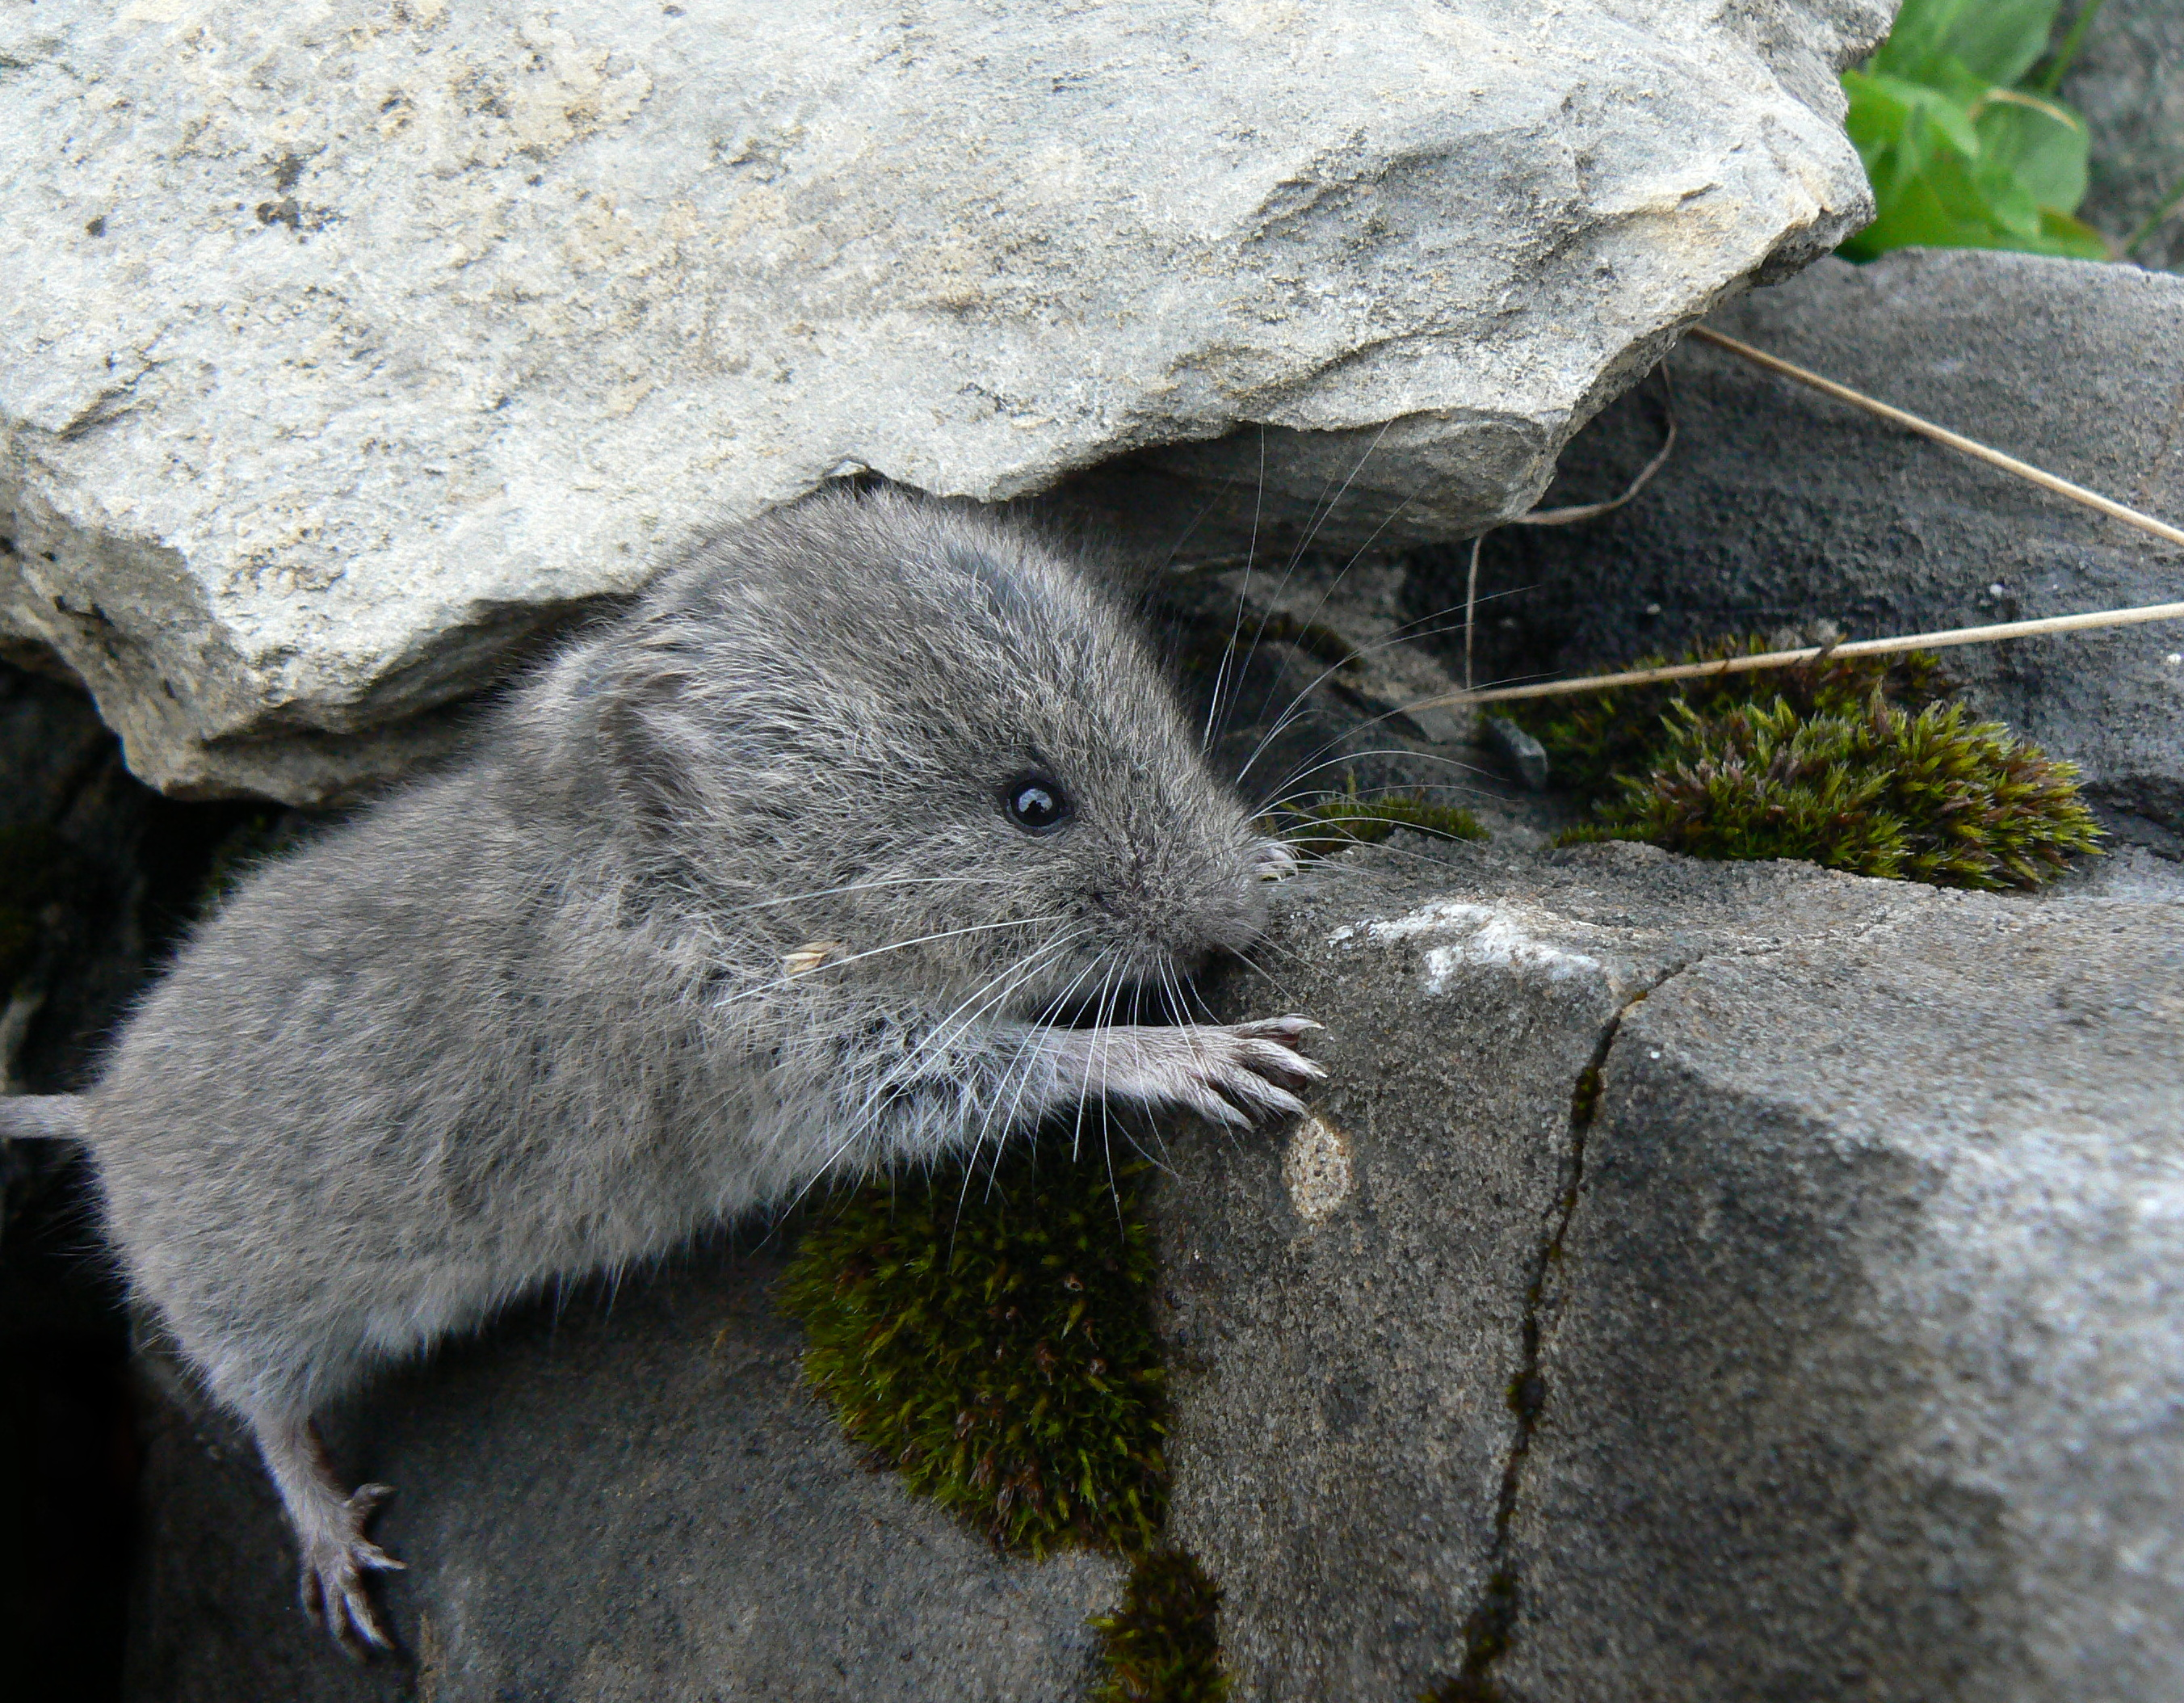
\includegraphics[width=0.45\textwidth]{Figures/cutevole}}}
%\subtitle{UOBU}
\author[\textbf{\fontfamily{pcr}\selectfont timothee.bonnet@ieu.uzh.ch}]{\textbf{Timoth\'{e}e Bonnet}}
%\date{\fcolorbox{blendedblue}{blendedblue}{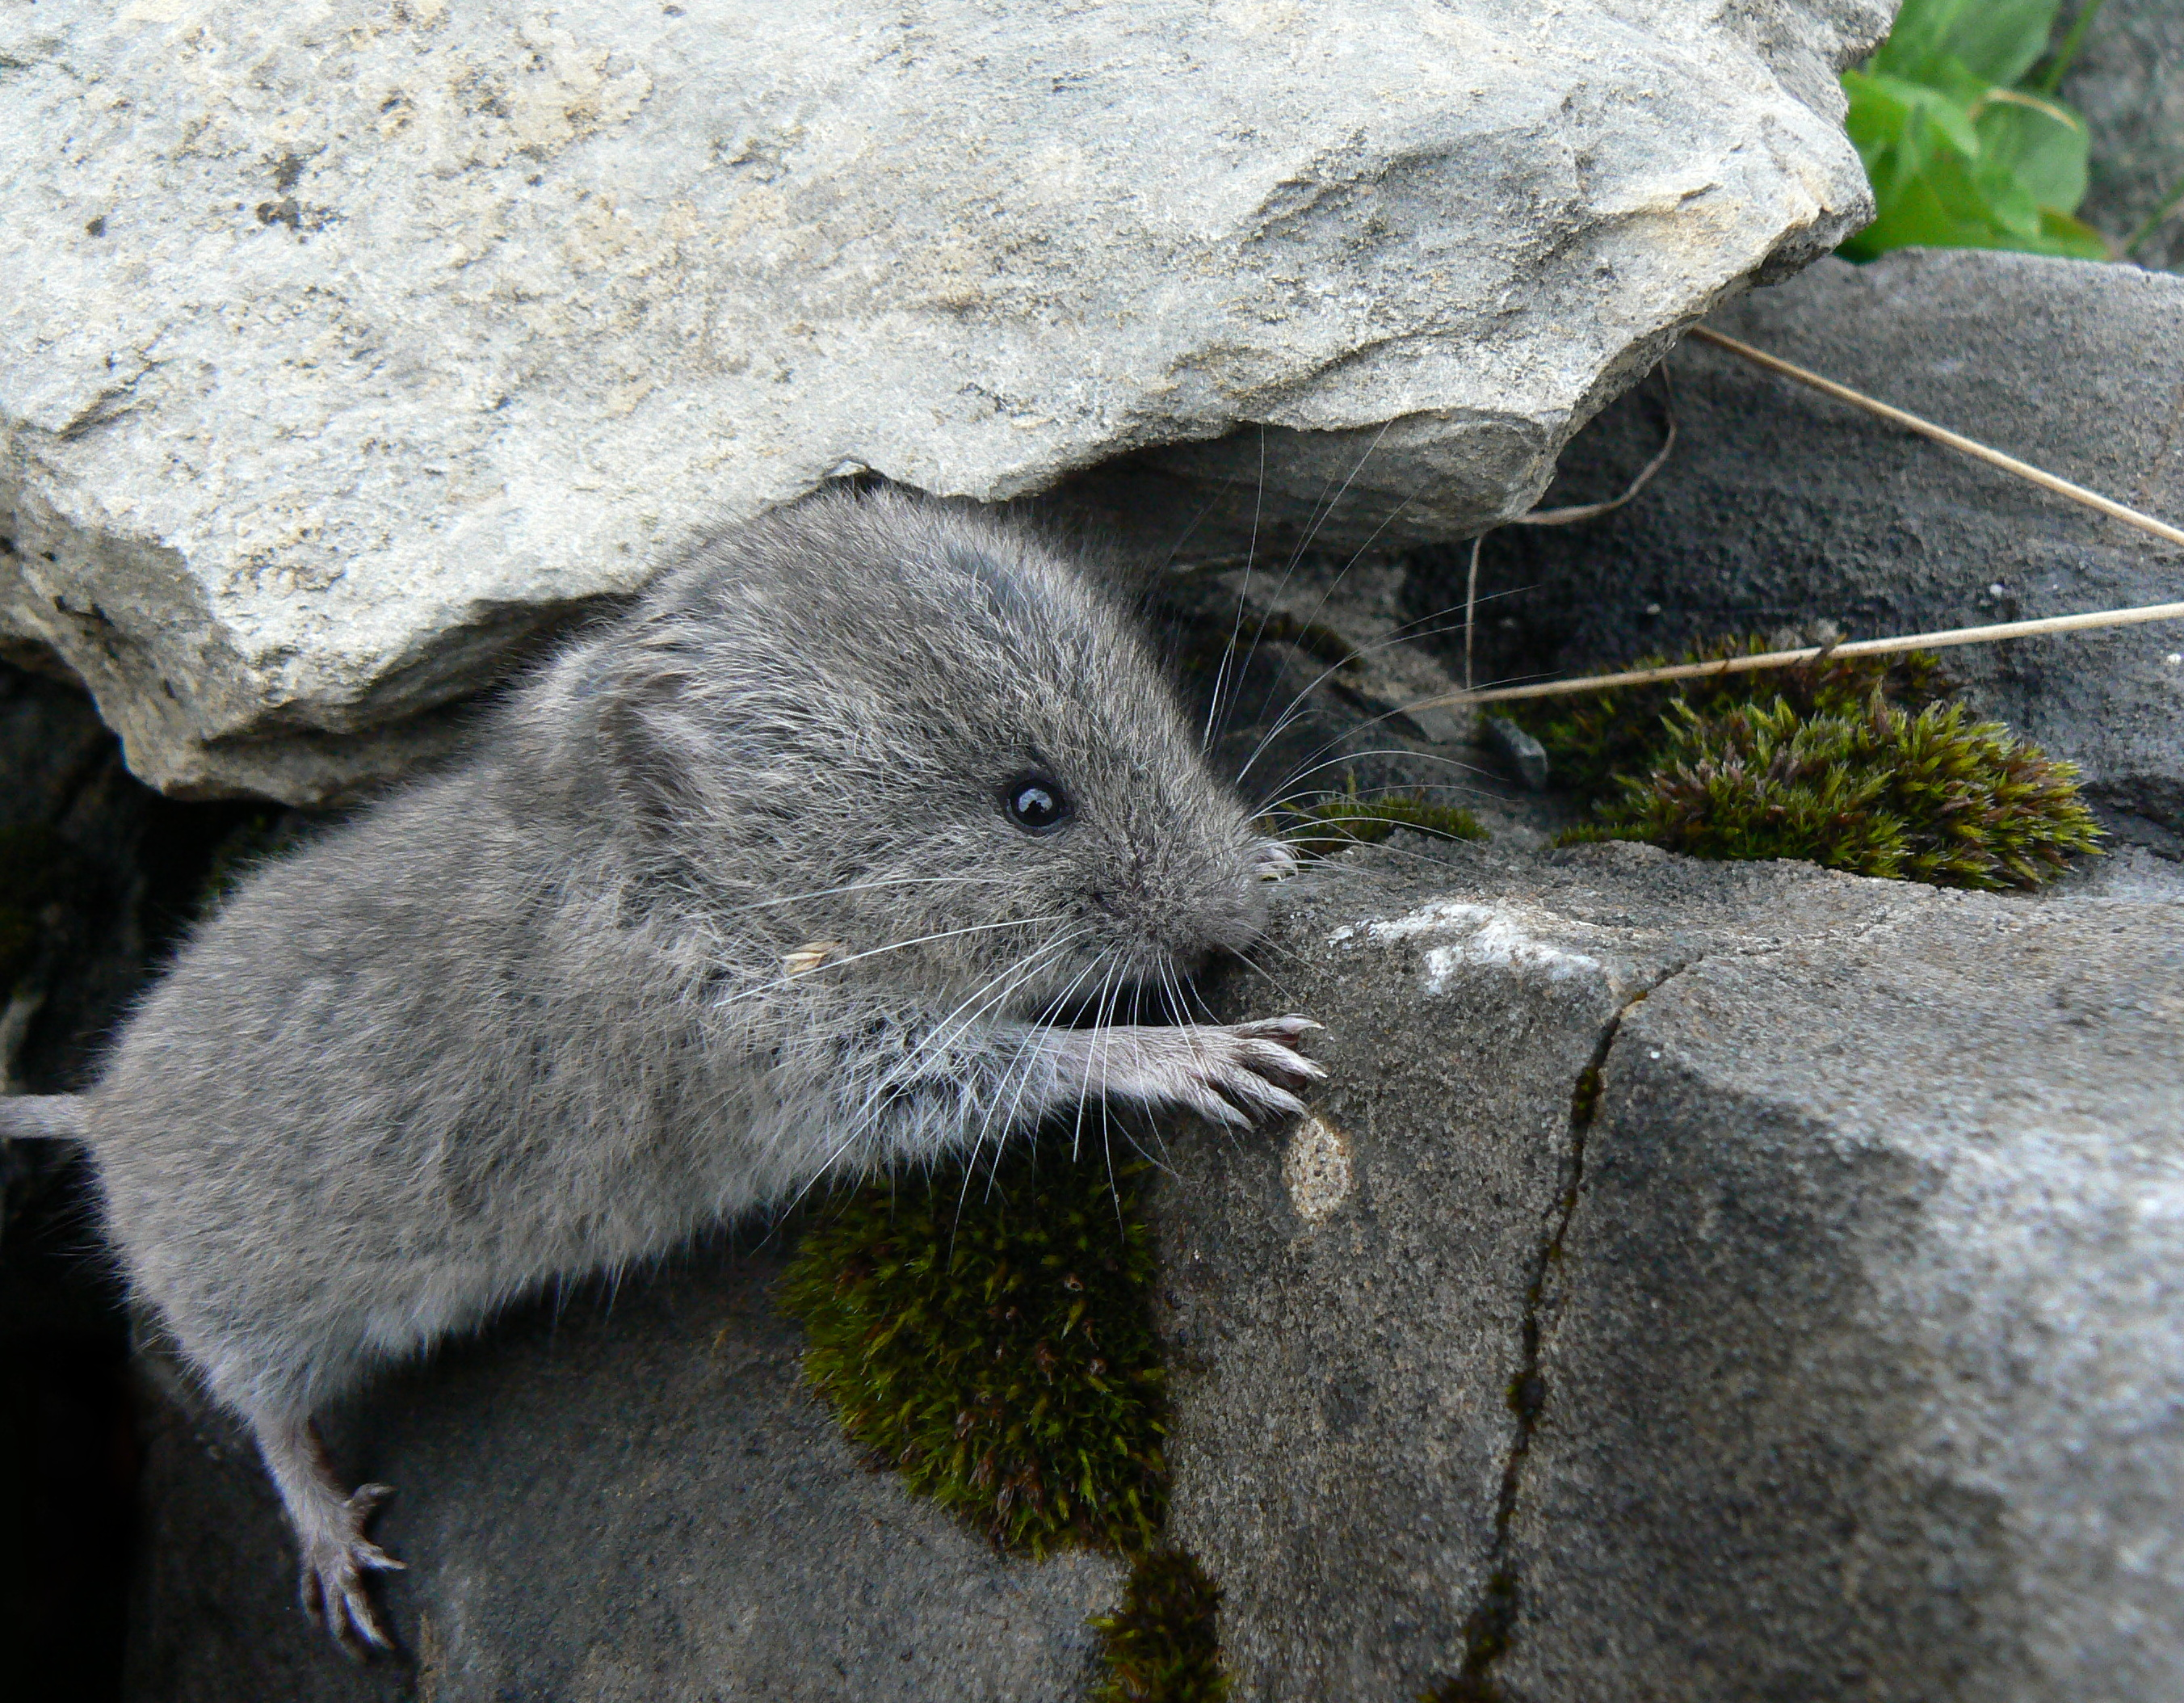
\includegraphics[width=0.35\textwidth]{Figures/cutevole}}}
\date{\vspace{1cm}}
\institute[IEU, University of Zurich]{\small Department of evolutionary biology and environmental studies (IEU) \\ \vspace{-0.1cm} \\ 
\includegraphics[width=0.3\textwidth]{Figures/uzhlogo}}



%%%%%%%%%%%%%%%%%%%%%%%%%%%%%%%%%%%%%%%%%%%%%%
\begin{document}

\begin{frame}[plain]
\maketitle
\end{frame}
%%%%%%%%%%%

\begin{frame}{These humans helped}

\begin{columns}
	\begin{column}[c]{0.33\textwidth}
		\begin{itemize}
			\item<2-> Erik Postma
		%committee
			\item<3-> Lukas Keller
			\item<3-> Barbara Tschirren
			\item<3-> Arpat Ozgul
			\item<3-> Marc Kéry 
			\item<3-> Jarrod Hadfield
		%colleagues
			\item<4-> Glauco Camenisch
			\item<5-> Ursina Tobler
			\item<6-> Dominique Waldvogel
			\item<6-> Martina Schenkel
					

%former colleagues?

%friends and family
		\end{itemize}
	\end{column}
	\begin{column}[c]{0.7\textwidth}
		%Residual
		\begin{figure}[c]
			\begin{tikzpicture}
				\uncover<2->{\node (erik) at (0,0) {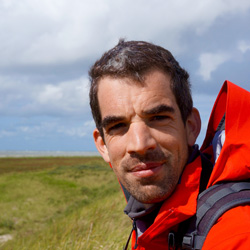
\includegraphics[width = 0.2 \textwidth]{Figures/Erik}};}
				\uncover<3->{\node (lukas) at (1.2,0) {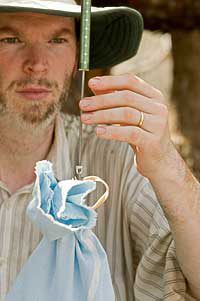
\includegraphics[width = 0.15 \textwidth]{Figures/Lukas}};
				\node (barbara) at (2.2,0) {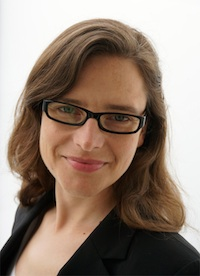
\includegraphics[width = 0.15 \textwidth]{Figures/Barbara}};
				\node (arpat) at (3.5,0) {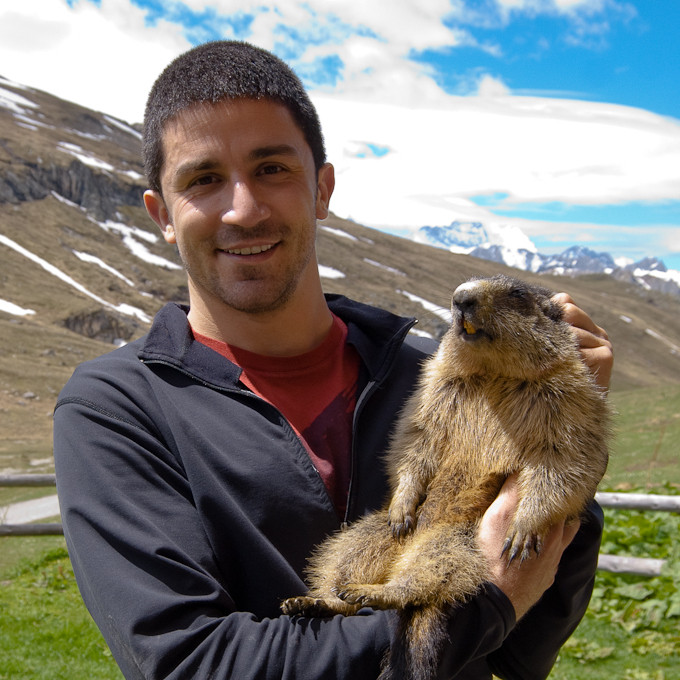
\includegraphics[width = 0.2 \textwidth]{Figures/Arpat}};
				\node (marc) at (4.7,0) {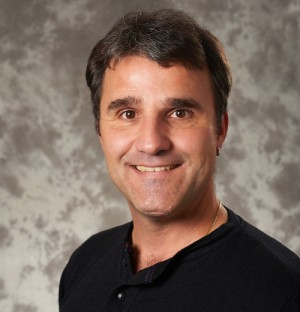
\includegraphics[width = 0.2 \textwidth]{Figures/Marc}};
				\node (jarrod) at (6,0) {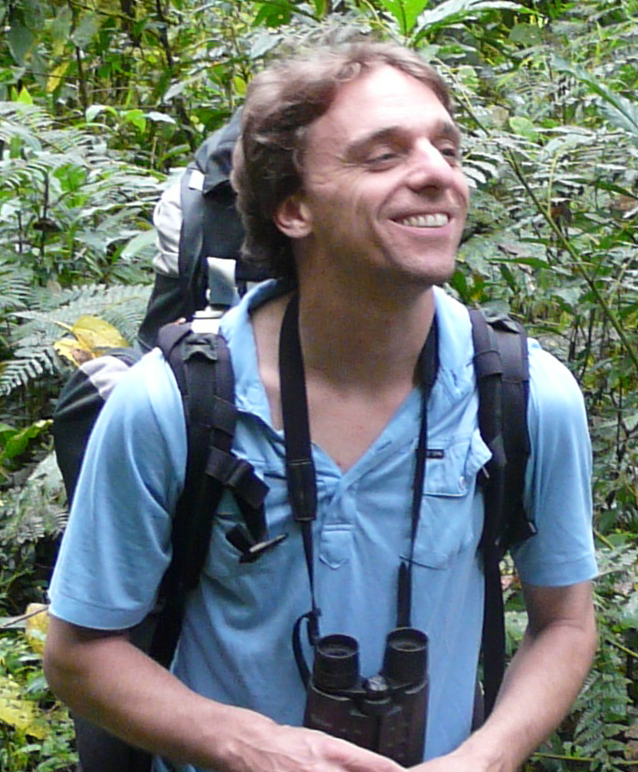
\includegraphics[width = 0.2\textwidth]{Figures/Jarrod}};}
				\uncover<4->{\node (glauco) at (0,-1.4) {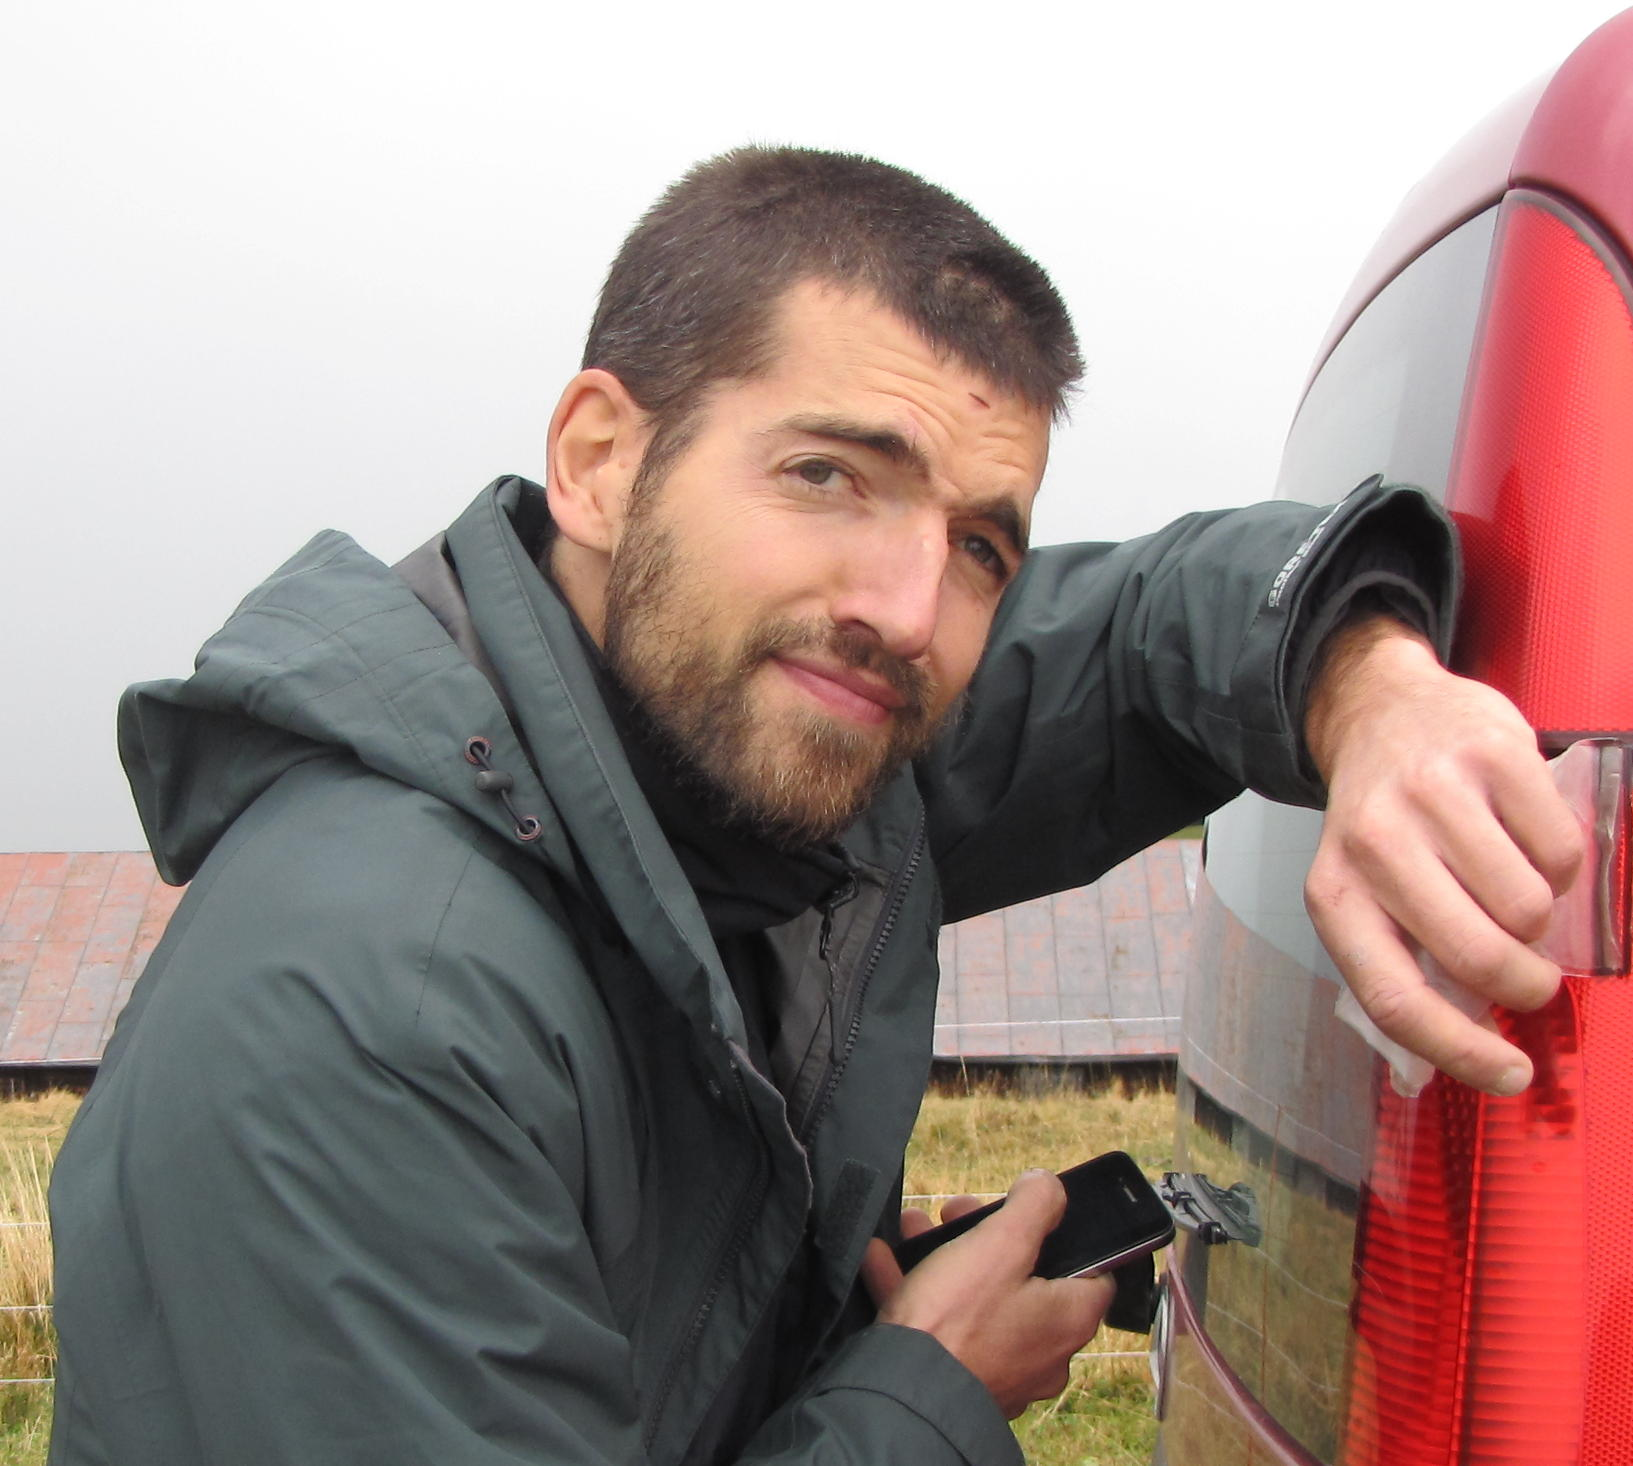
\includegraphics[width = 0.22 \textwidth]{Figures/Glauco}};}
				\uncover<5->{\node (ursina) at (1.2,-1.4) {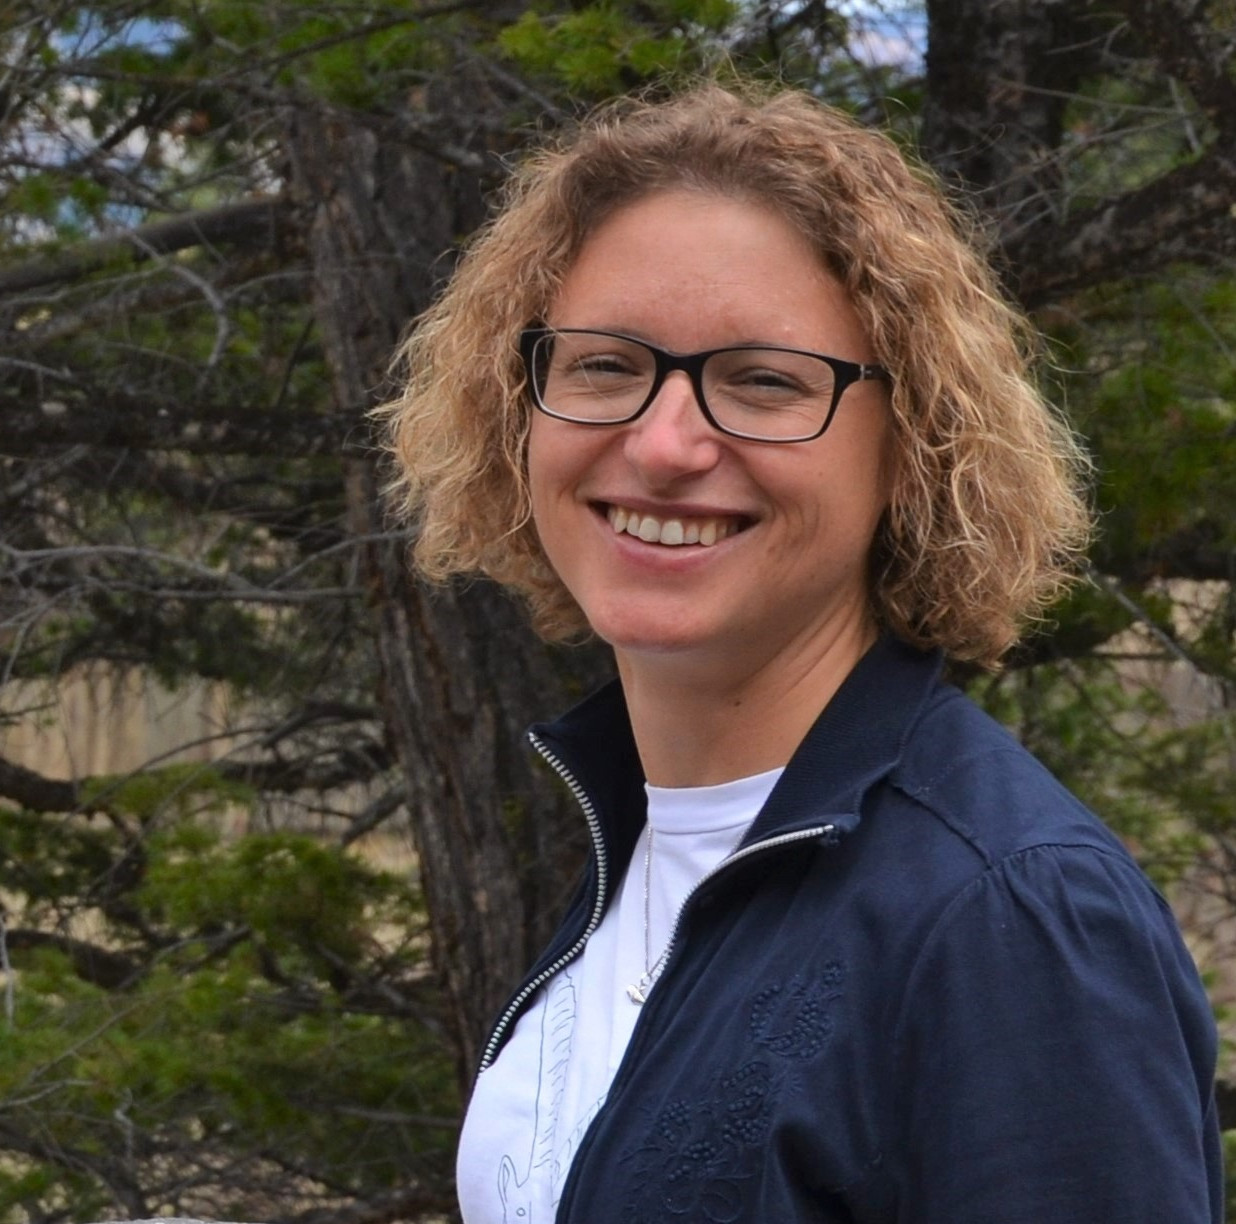
\includegraphics[width = 0.20 \textwidth]{Figures/Ursina}};}
				\uncover<6->{\node (domi) at (2.6,-1.4) {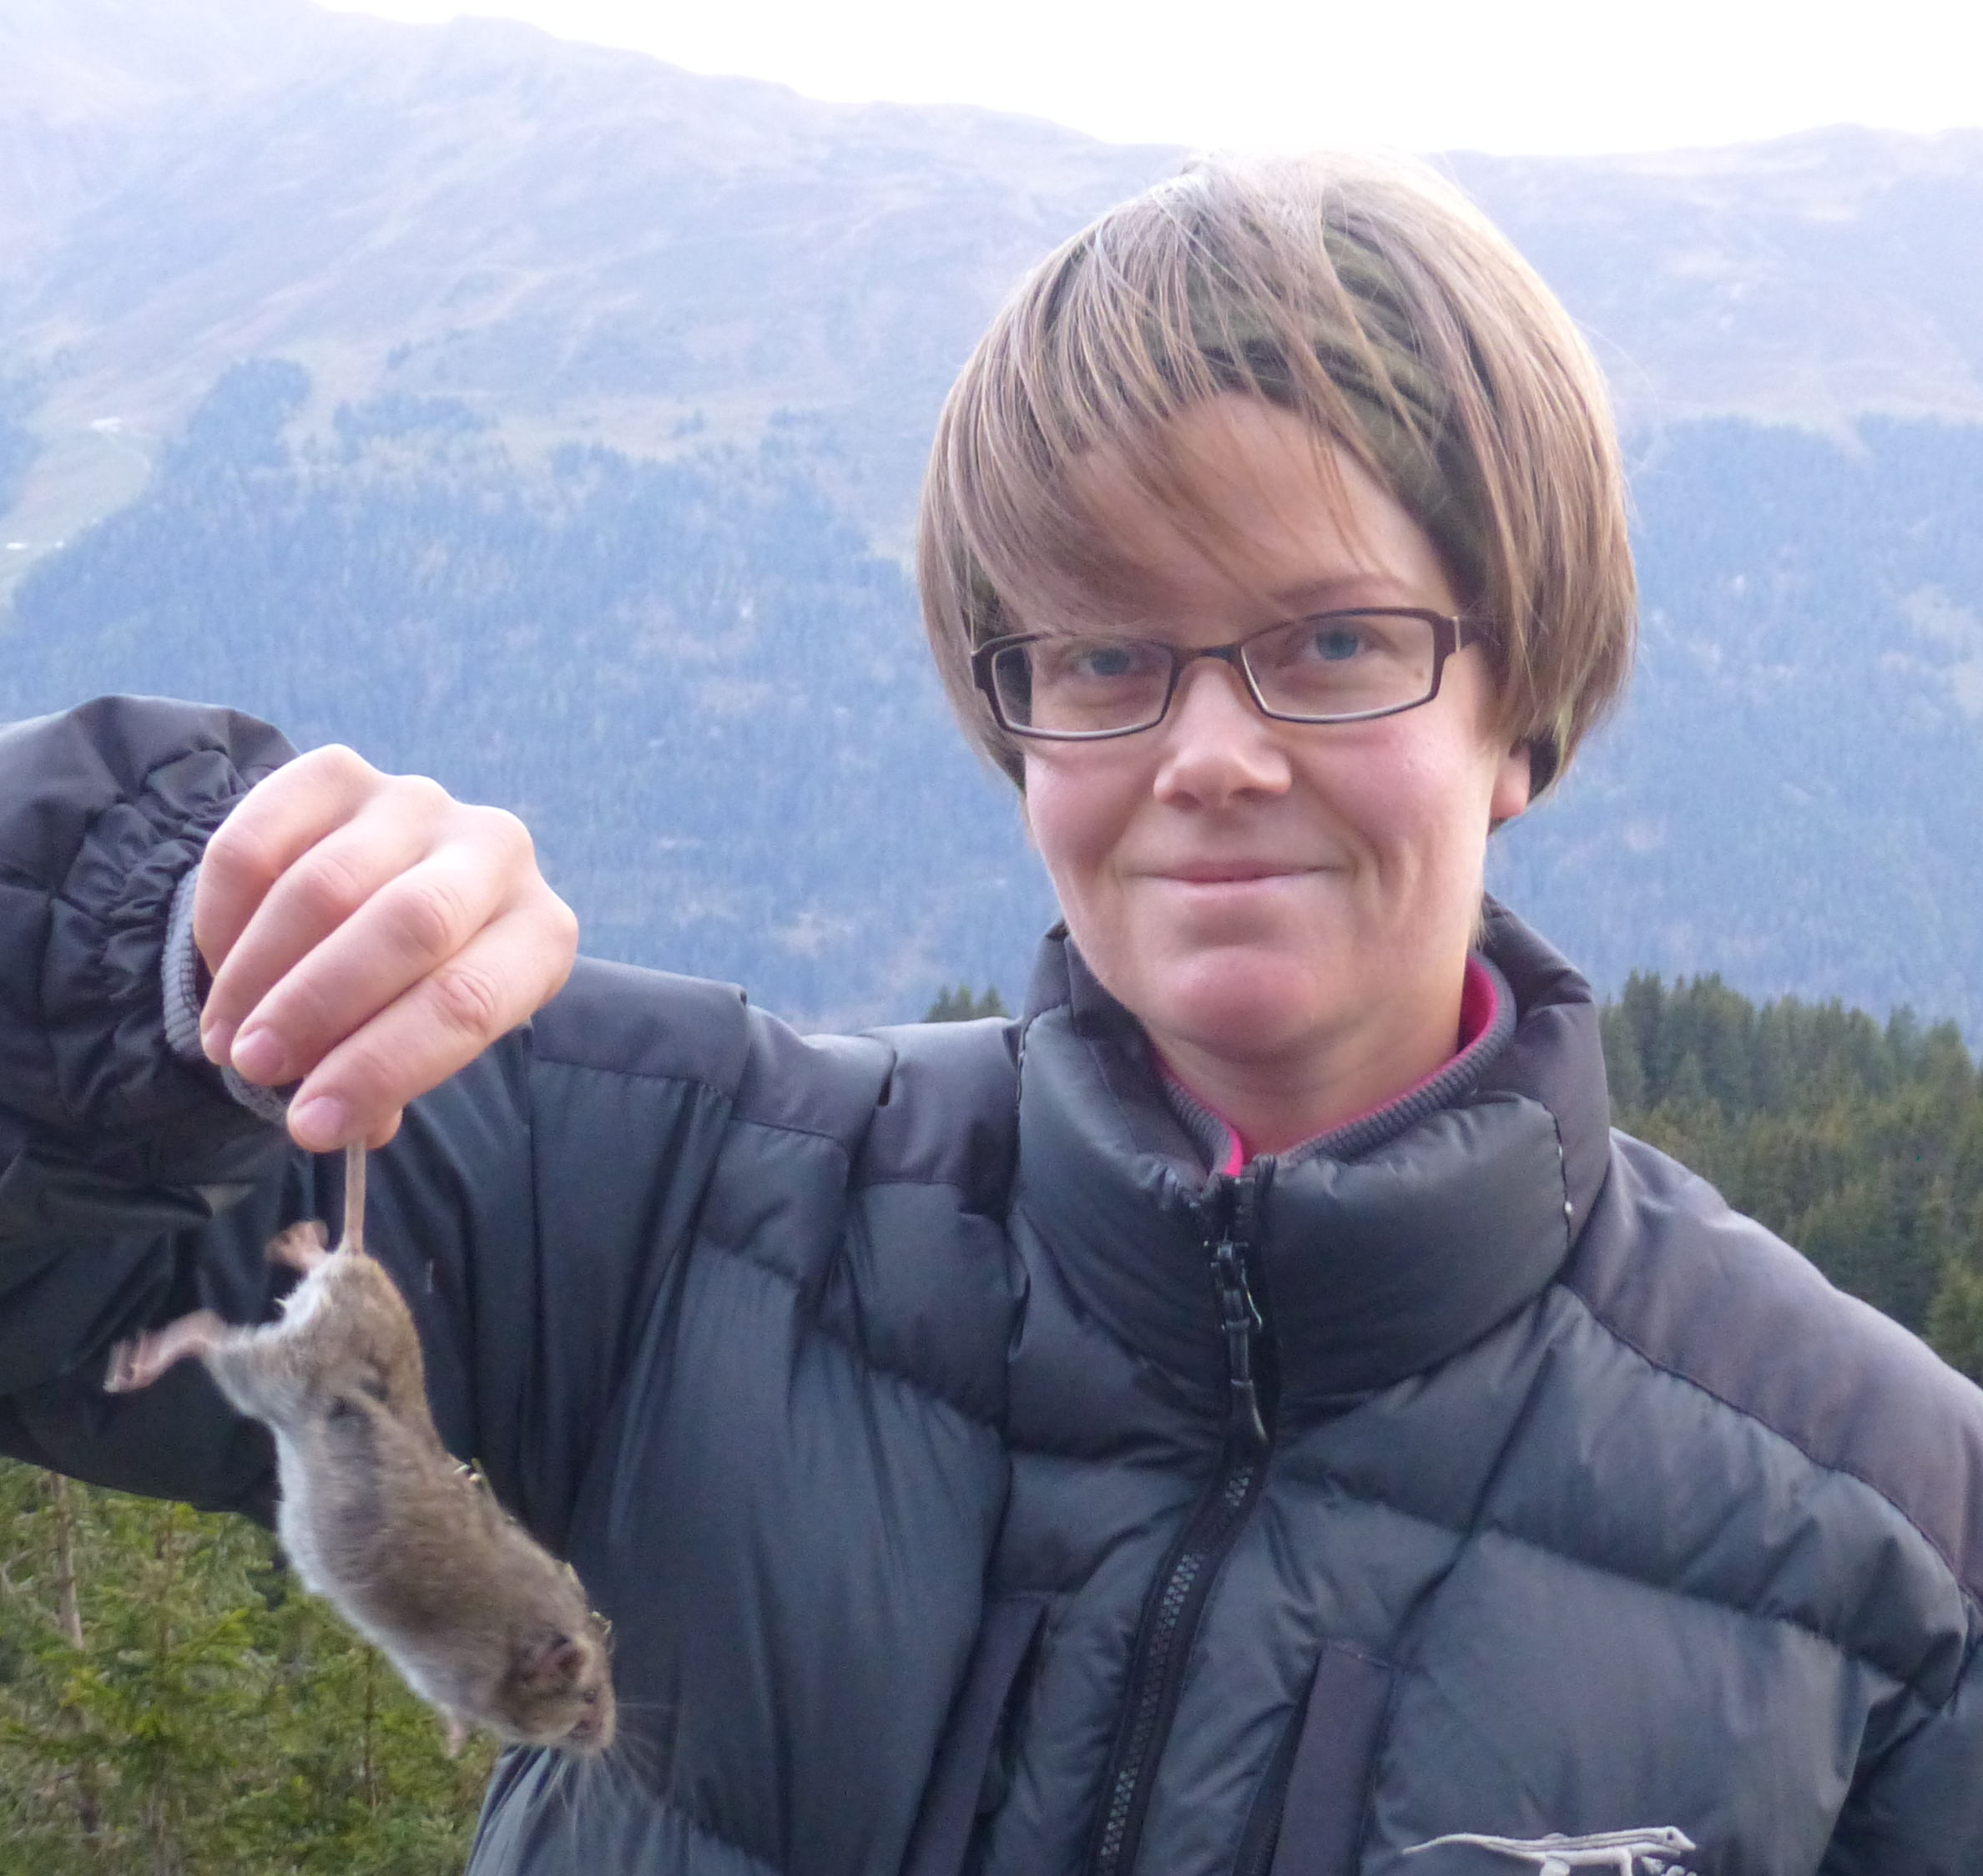
\includegraphics[width = 0.20 \textwidth]{Figures/Domi}};}
				\uncover<6->{\node (martina) at (3.8,-1.4) {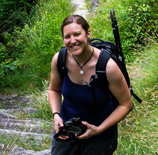
\includegraphics[width = 0.17 \textwidth]{Figures/Martina}};}
				
			\end{tikzpicture}
		\end{figure}
	\end{column}
\end{columns}

\end{frame}
%%%%%%%%%%%

%Acknowledgements

%Intro on variation within species/population
%Explain causes of variation imply consequences



%%%%%%%%%%%%%%%%%%%%%%%%%%%%%%%%%%%%%%%%%%%%%%%%%%%%%%
%%%%%%%%%%%%%%%%%%%%%%% Chap 1 %%%%%%%%%%%%%%%%%%%%%%%
%%%%%%%%%%%%%%%%%%%%%%%%%%%%%%%%%%%%%%%%%%%%%%%%%%%%%%
%Dice!

%%%%%%%%%%%%%%%%%%%%%%%%%%%%%%%%%%%%%%%%%%%%%%%%%%%%%%
%%%%%%%%%%%%%%%%%%%%%%% Chap 2 %%%%%%%%%%%%%%%%%%%%%%%
%%%%%%%%%%%%%%%%%%%%%%%%%%%%%%%%%%%%%%%%%%%%%%%%%%%%%%



%FIeld and population
\begin{frame}[plain]{}
	\begin{figure}
	\centering
		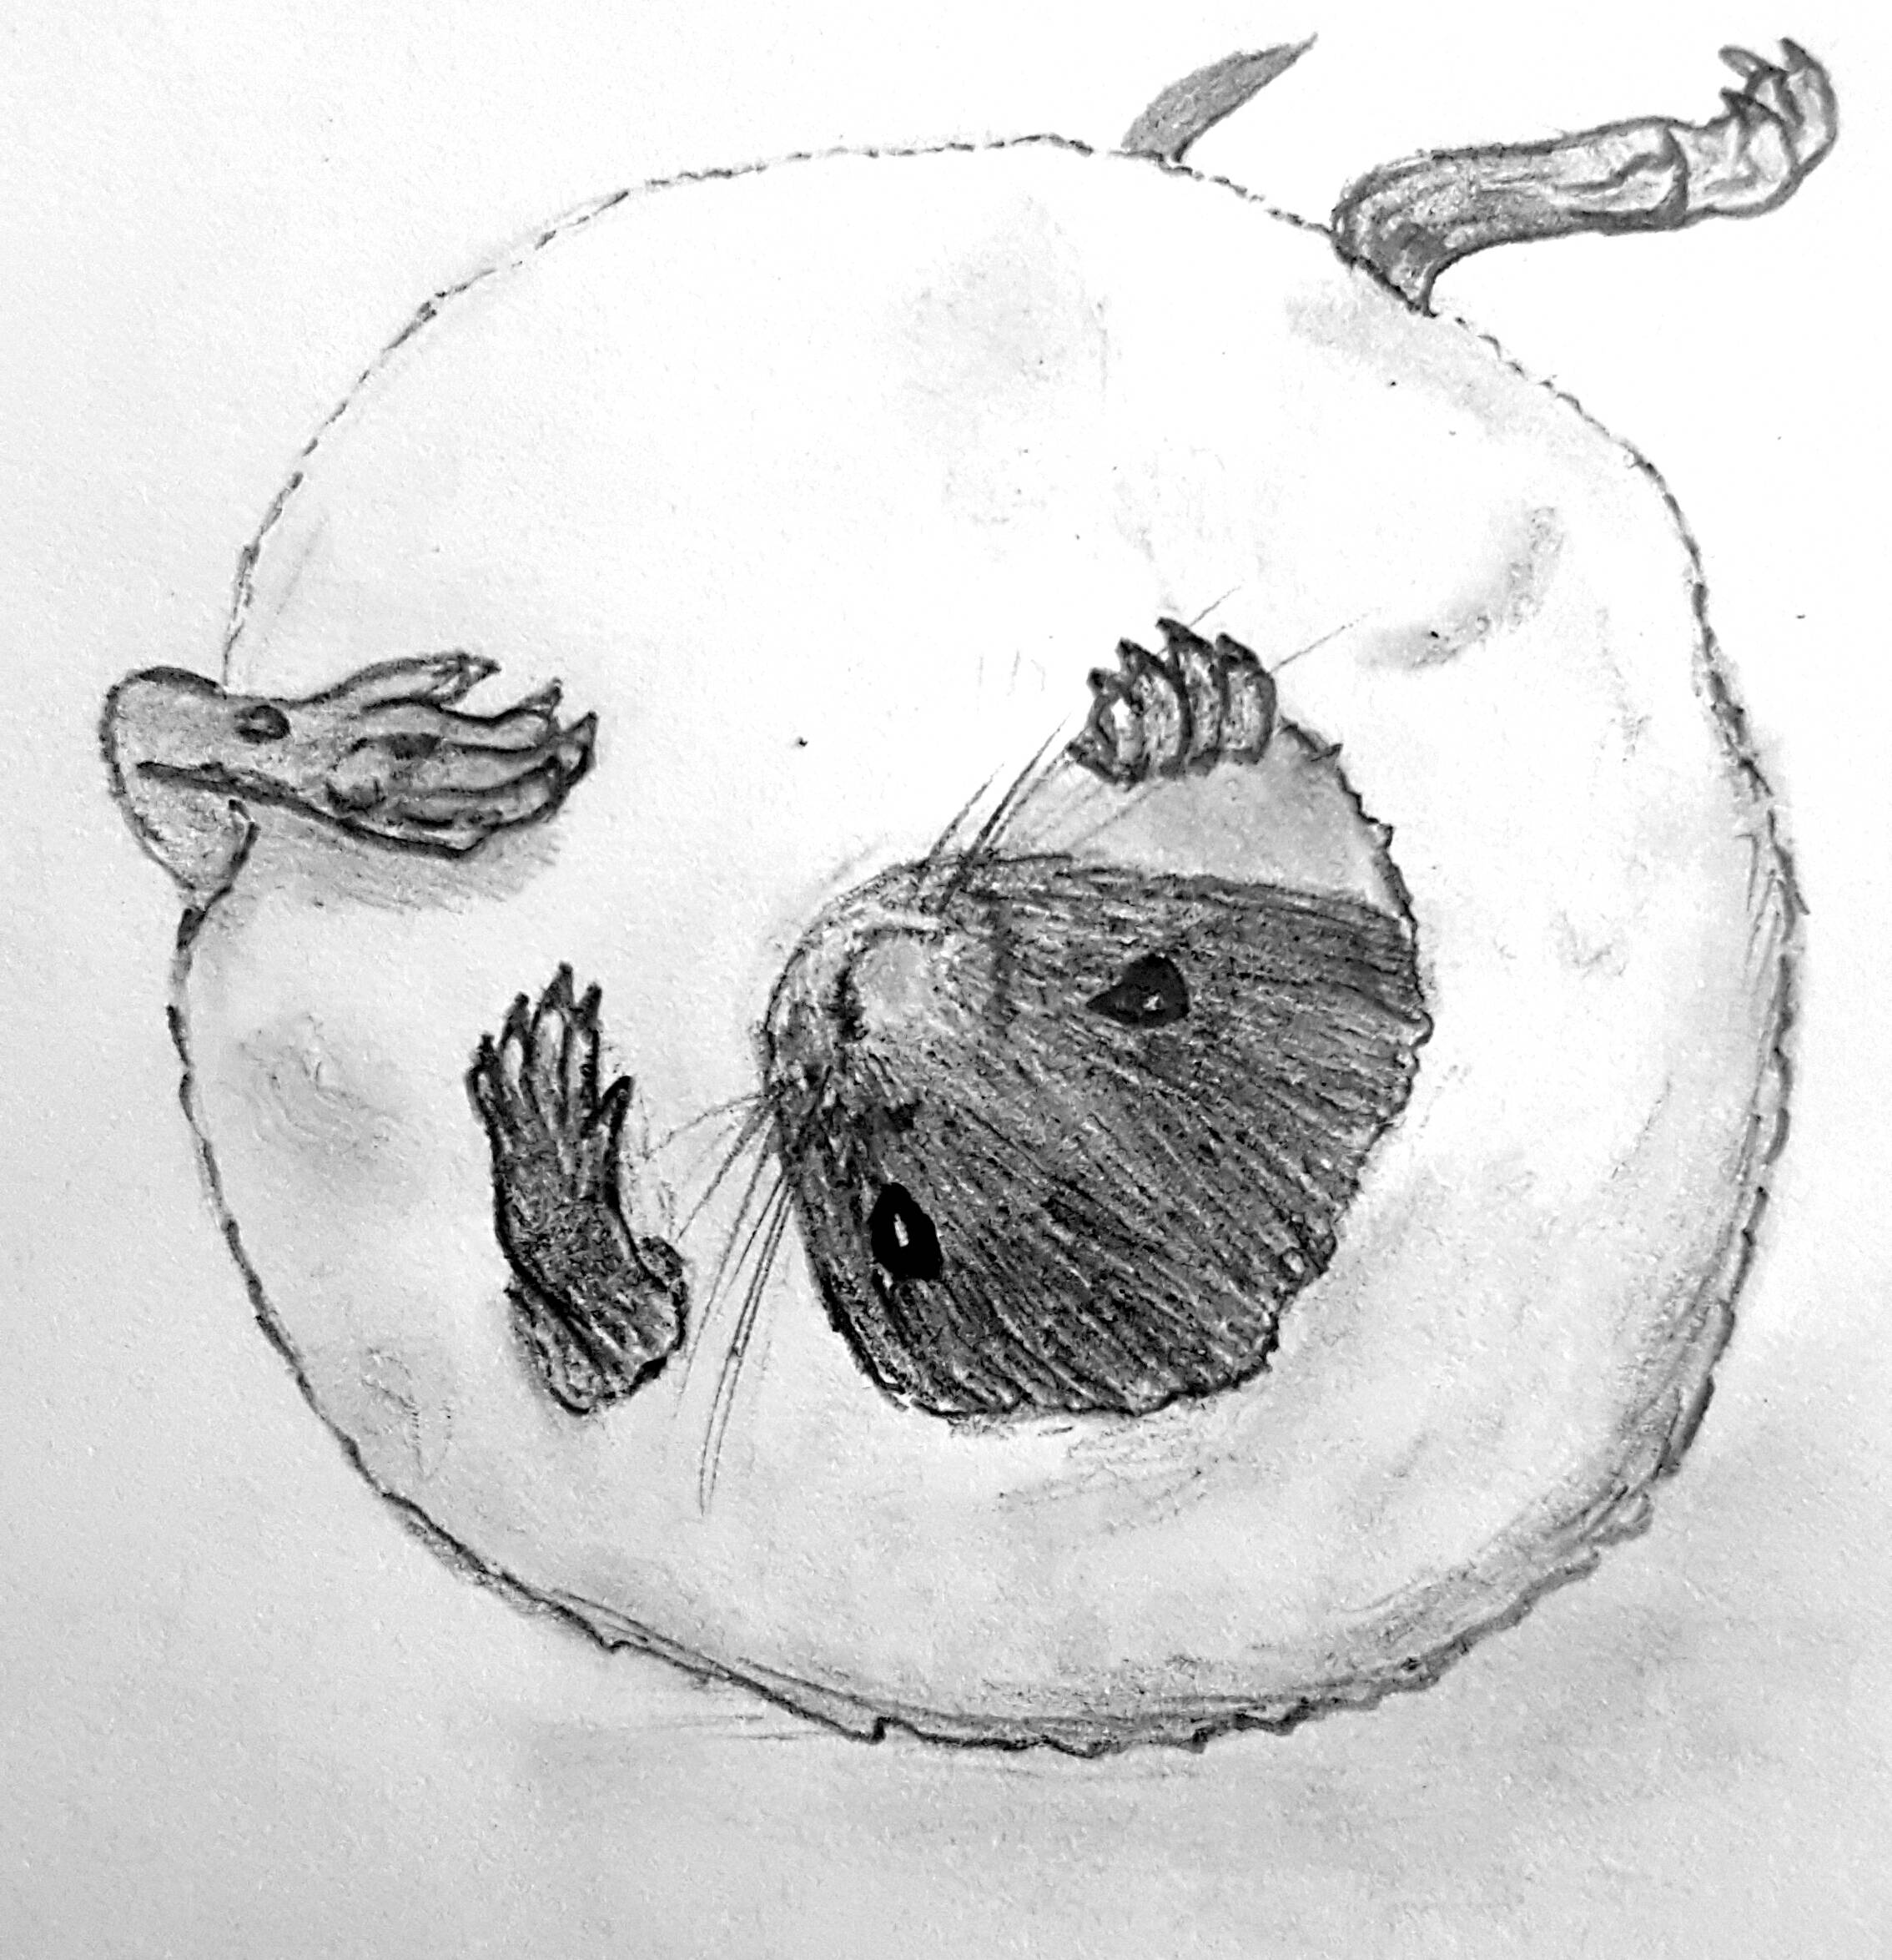
\includegraphics[height= \textheight]{Figures/SnowBall}
	\end{figure}
\end{frame}
%%%%%%%%%%%

\begin{frame}{Snow vole (\textit{Chionomys nivalis}, Martins 1842)}

\begin{columns}
	\begin{column}[c]{0.5\textwidth}
		\begin{itemize}[<+->]
			\item NOT white
			\item Rock-dweller
			\item 30-45g
			\item 10-14cm long $+$ 5-8cm tail
			\item Slow life pace
		\end{itemize}
	\end{column}
	\begin{column}[c]{0.5\textwidth}
	\begin{figure}
	\centering
		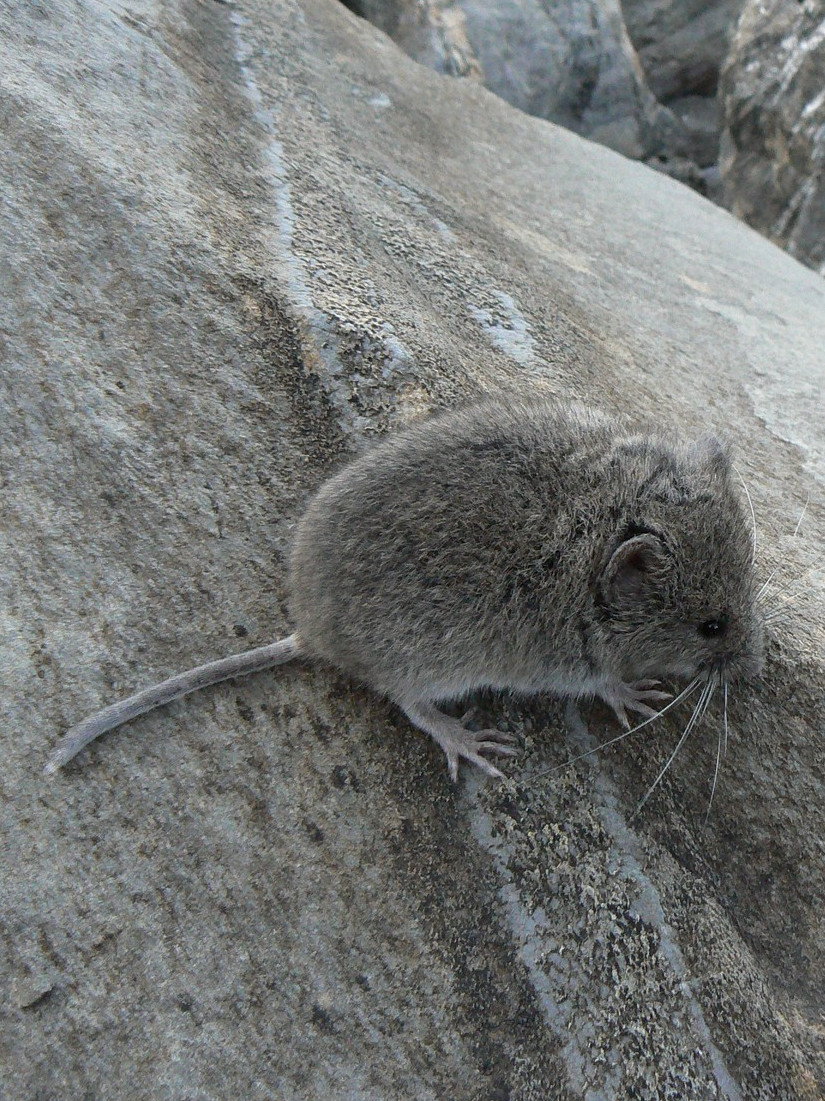
\includegraphics[width= \textwidth]{Figures/P1250035}
	\end{figure}
	\end{column}
	\end{columns}
\end{frame}
%%%%%%%%%%%



\begin{frame}[plain]{}
	\begin{figure}
	\centering
		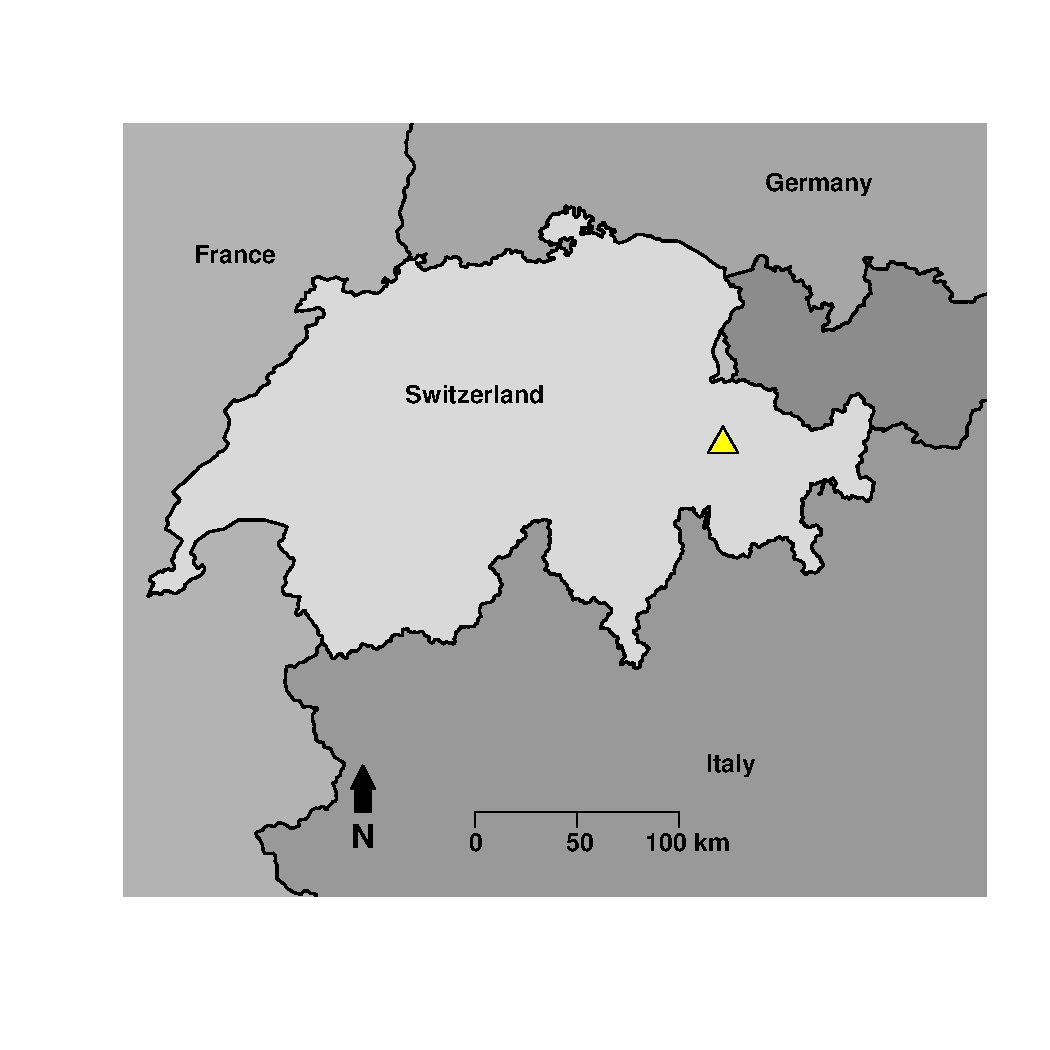
\includegraphics[height= \textheight]{Figures/map-1}
	\end{figure}
\end{frame}
%%%%%%%%%%%

\begin{frame}[plain]{}
	\begin{figure}
	\centering
		\begin{tikzpicture}
			
			\node (pic) at (0,0) {\includegraphics[width= 0.95\textwidth]{Figures/DSC_2111viewontaliflue}};
			\draw[rounded corners,thick,color=red] (-1.2,-0.8) rectangle (0.5,0);
		\end{tikzpicture}
	\end{figure}
\end{frame}
%%%%%%%%%%%

\begin{frame}[plain]{}
	\begin{figure}
	\centering
		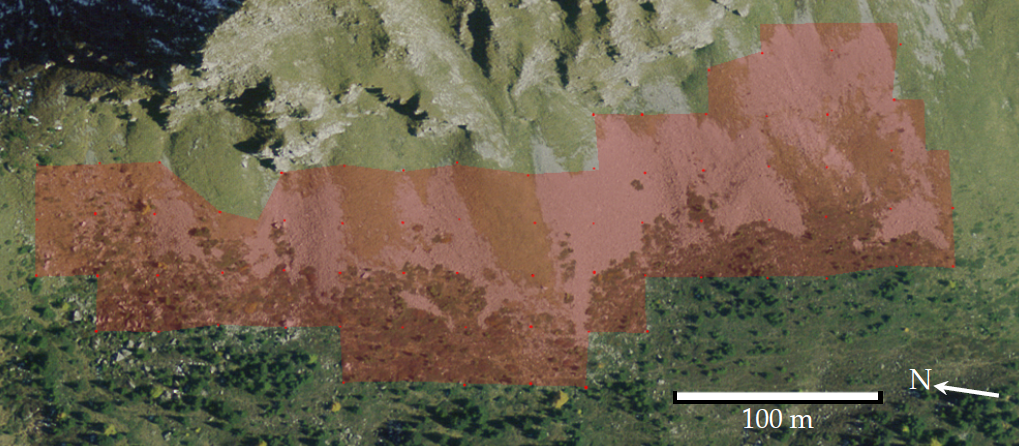
\includegraphics[width= \textwidth]{Figures/fieldposts2}
	\end{figure}
\end{frame}
%%%%%%%%%%%

\begin{frame}[plain]{}
	\begin{figure}
	\centering
		\includegraphics[width= \textwidth]{Figures/boulder}
	\end{figure}
\end{frame}
%%%%%%%%%%%

\begin{frame}[plain]{}
	\begin{figure}
	\centering
		\includegraphics[width= \textwidth]{Figures/DSC_2027trap}
	\end{figure}
\end{frame}
%%%%%%%%%%%

\begin{frame}{What we measure}

\begin{columns}
	\begin{column}[c]{0.4\textwidth}
		\begin{itemize}
			\item<2-> Morphology
				\begin{itemize}
					\item Body mass 
					\item Body length
					\item Tail length
				\end{itemize}
			\item<3-> Capture/Recaptures
				\begin{itemize}
					\item Death/emigration
					\item Location
				\end{itemize}
			\item<4-> DNA
				\begin{itemize}
					\item 20 ``neutral'' markers
					\item Sex identification
					\item Any genotyping
					\item<5-> \textbf{Pedigree}
				\end{itemize}
		\end{itemize}
	\end{column}
	
	\begin{column}[c]{0.6\textwidth}

	\centering
		\only<2>{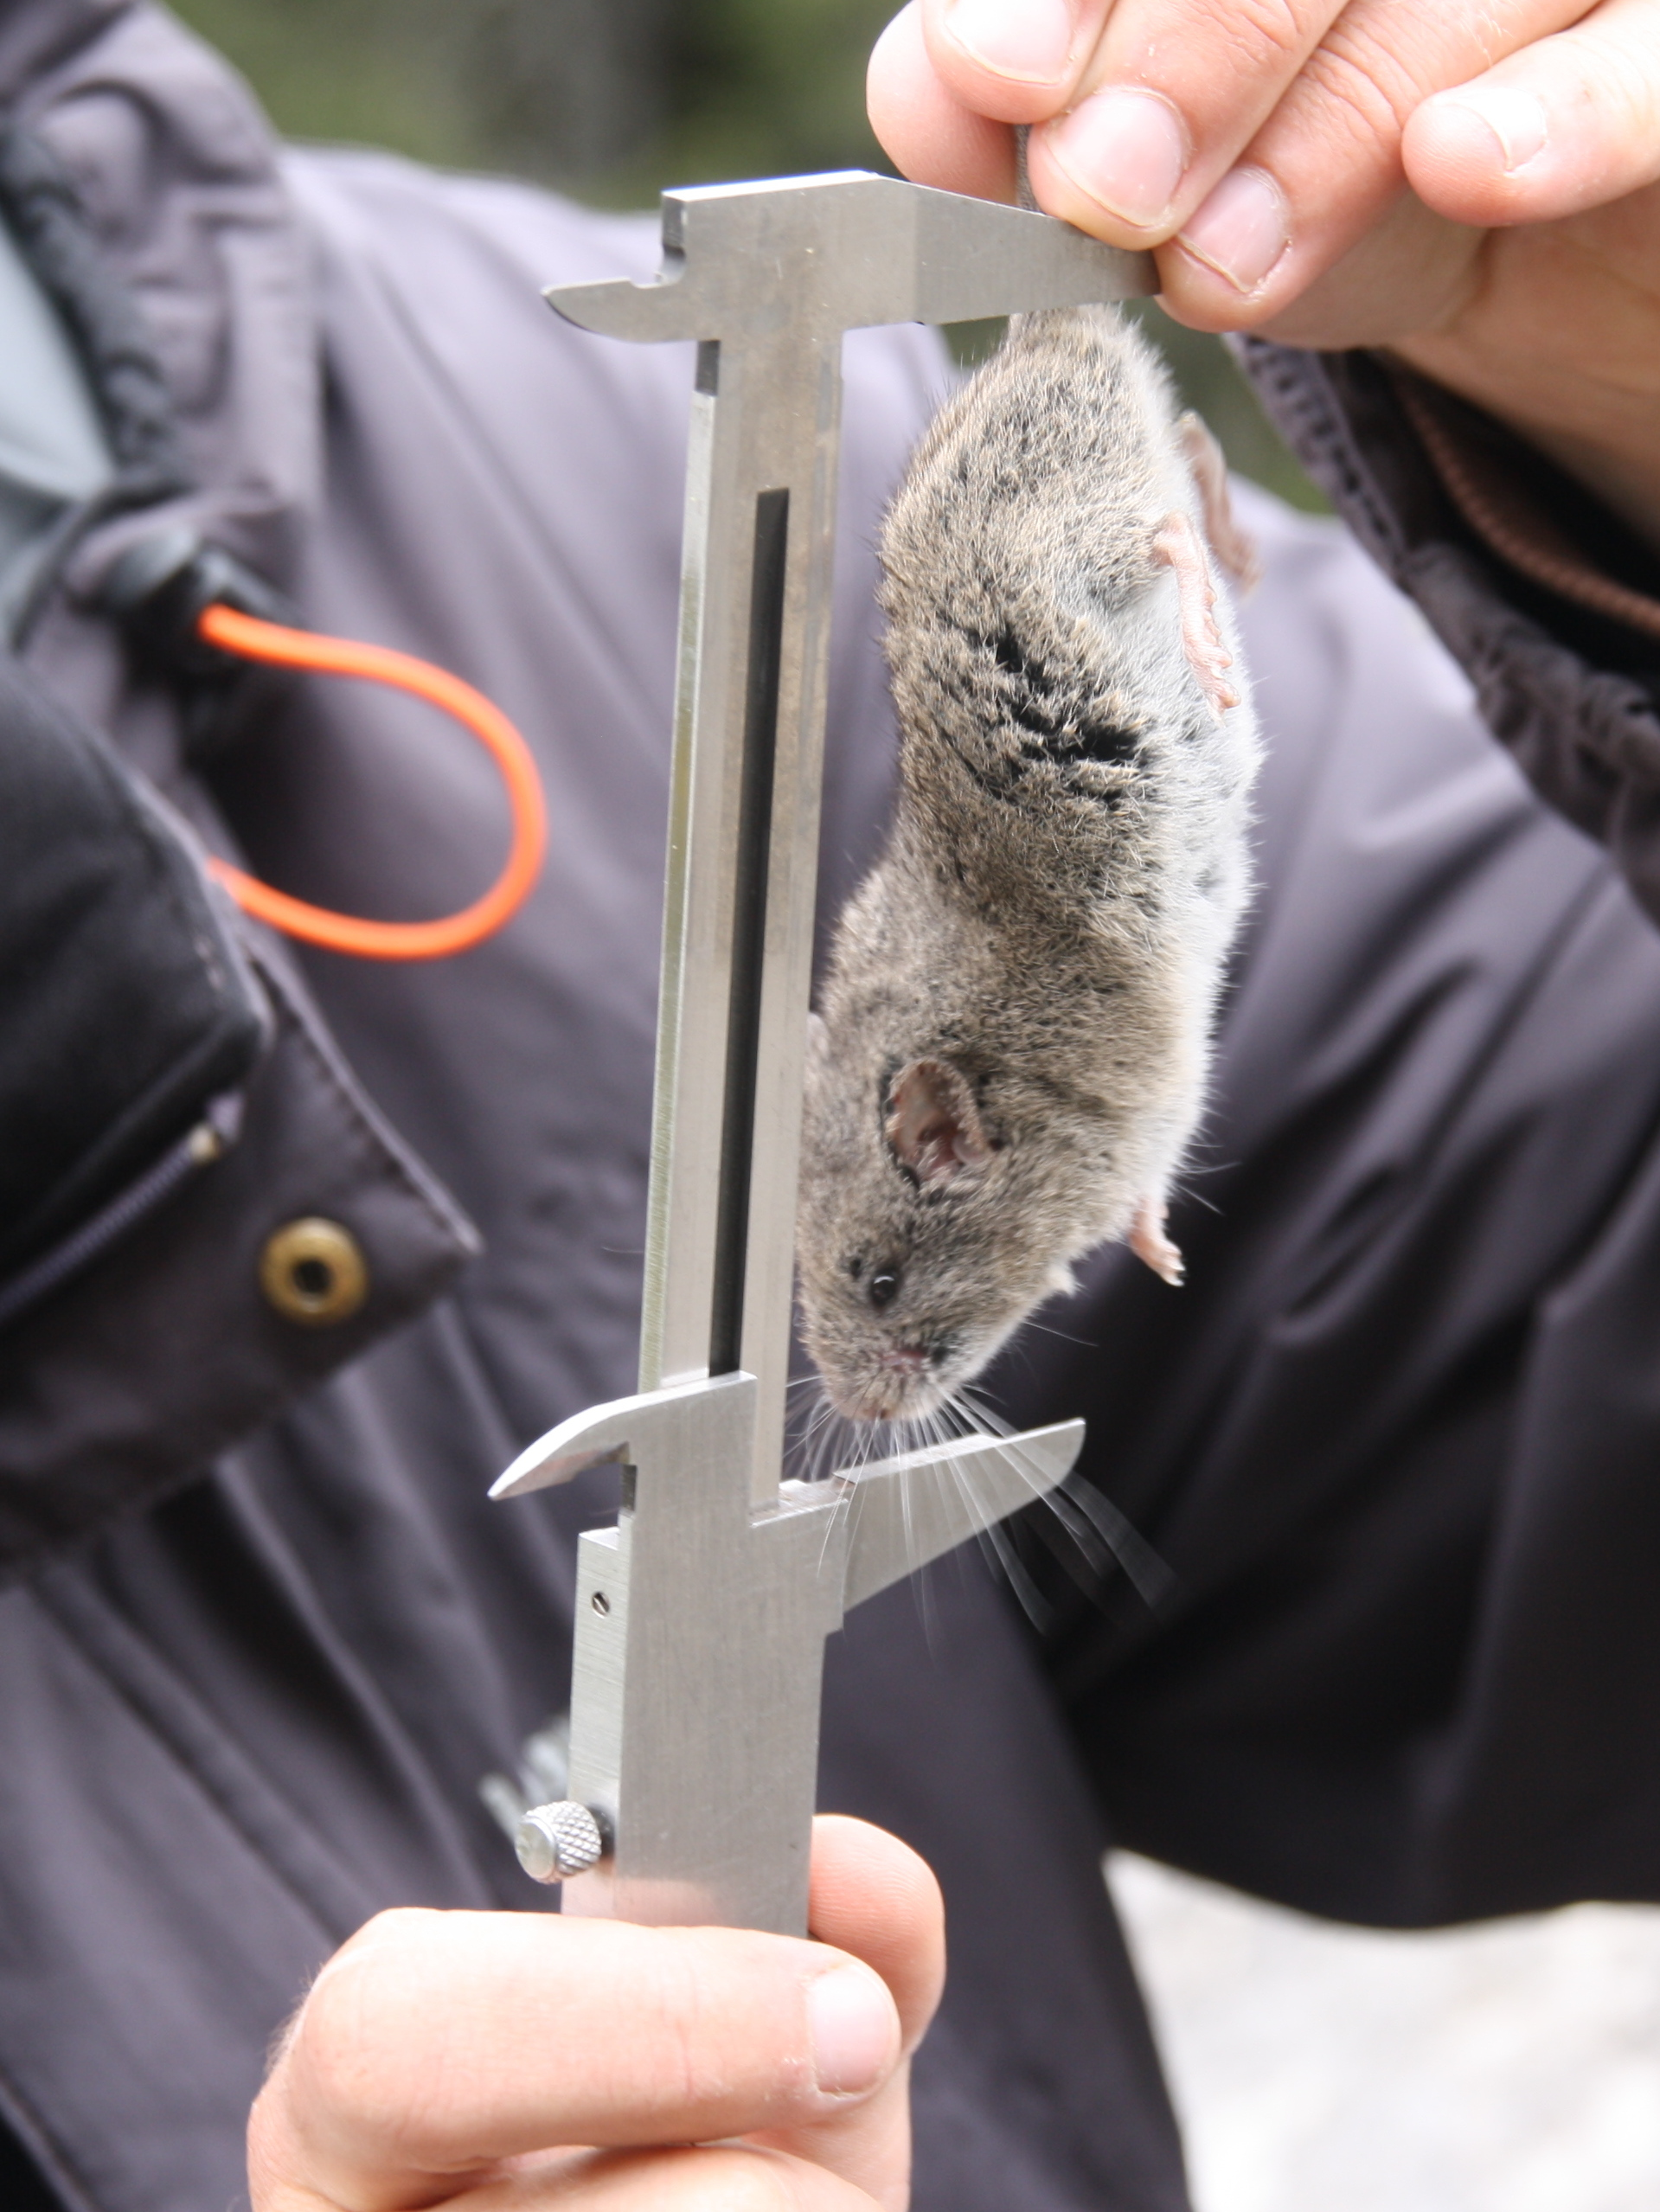
\includegraphics[height= \textheight]{Figures/CN2015_MeulenbroekLiz_00024}}
		\only<3>{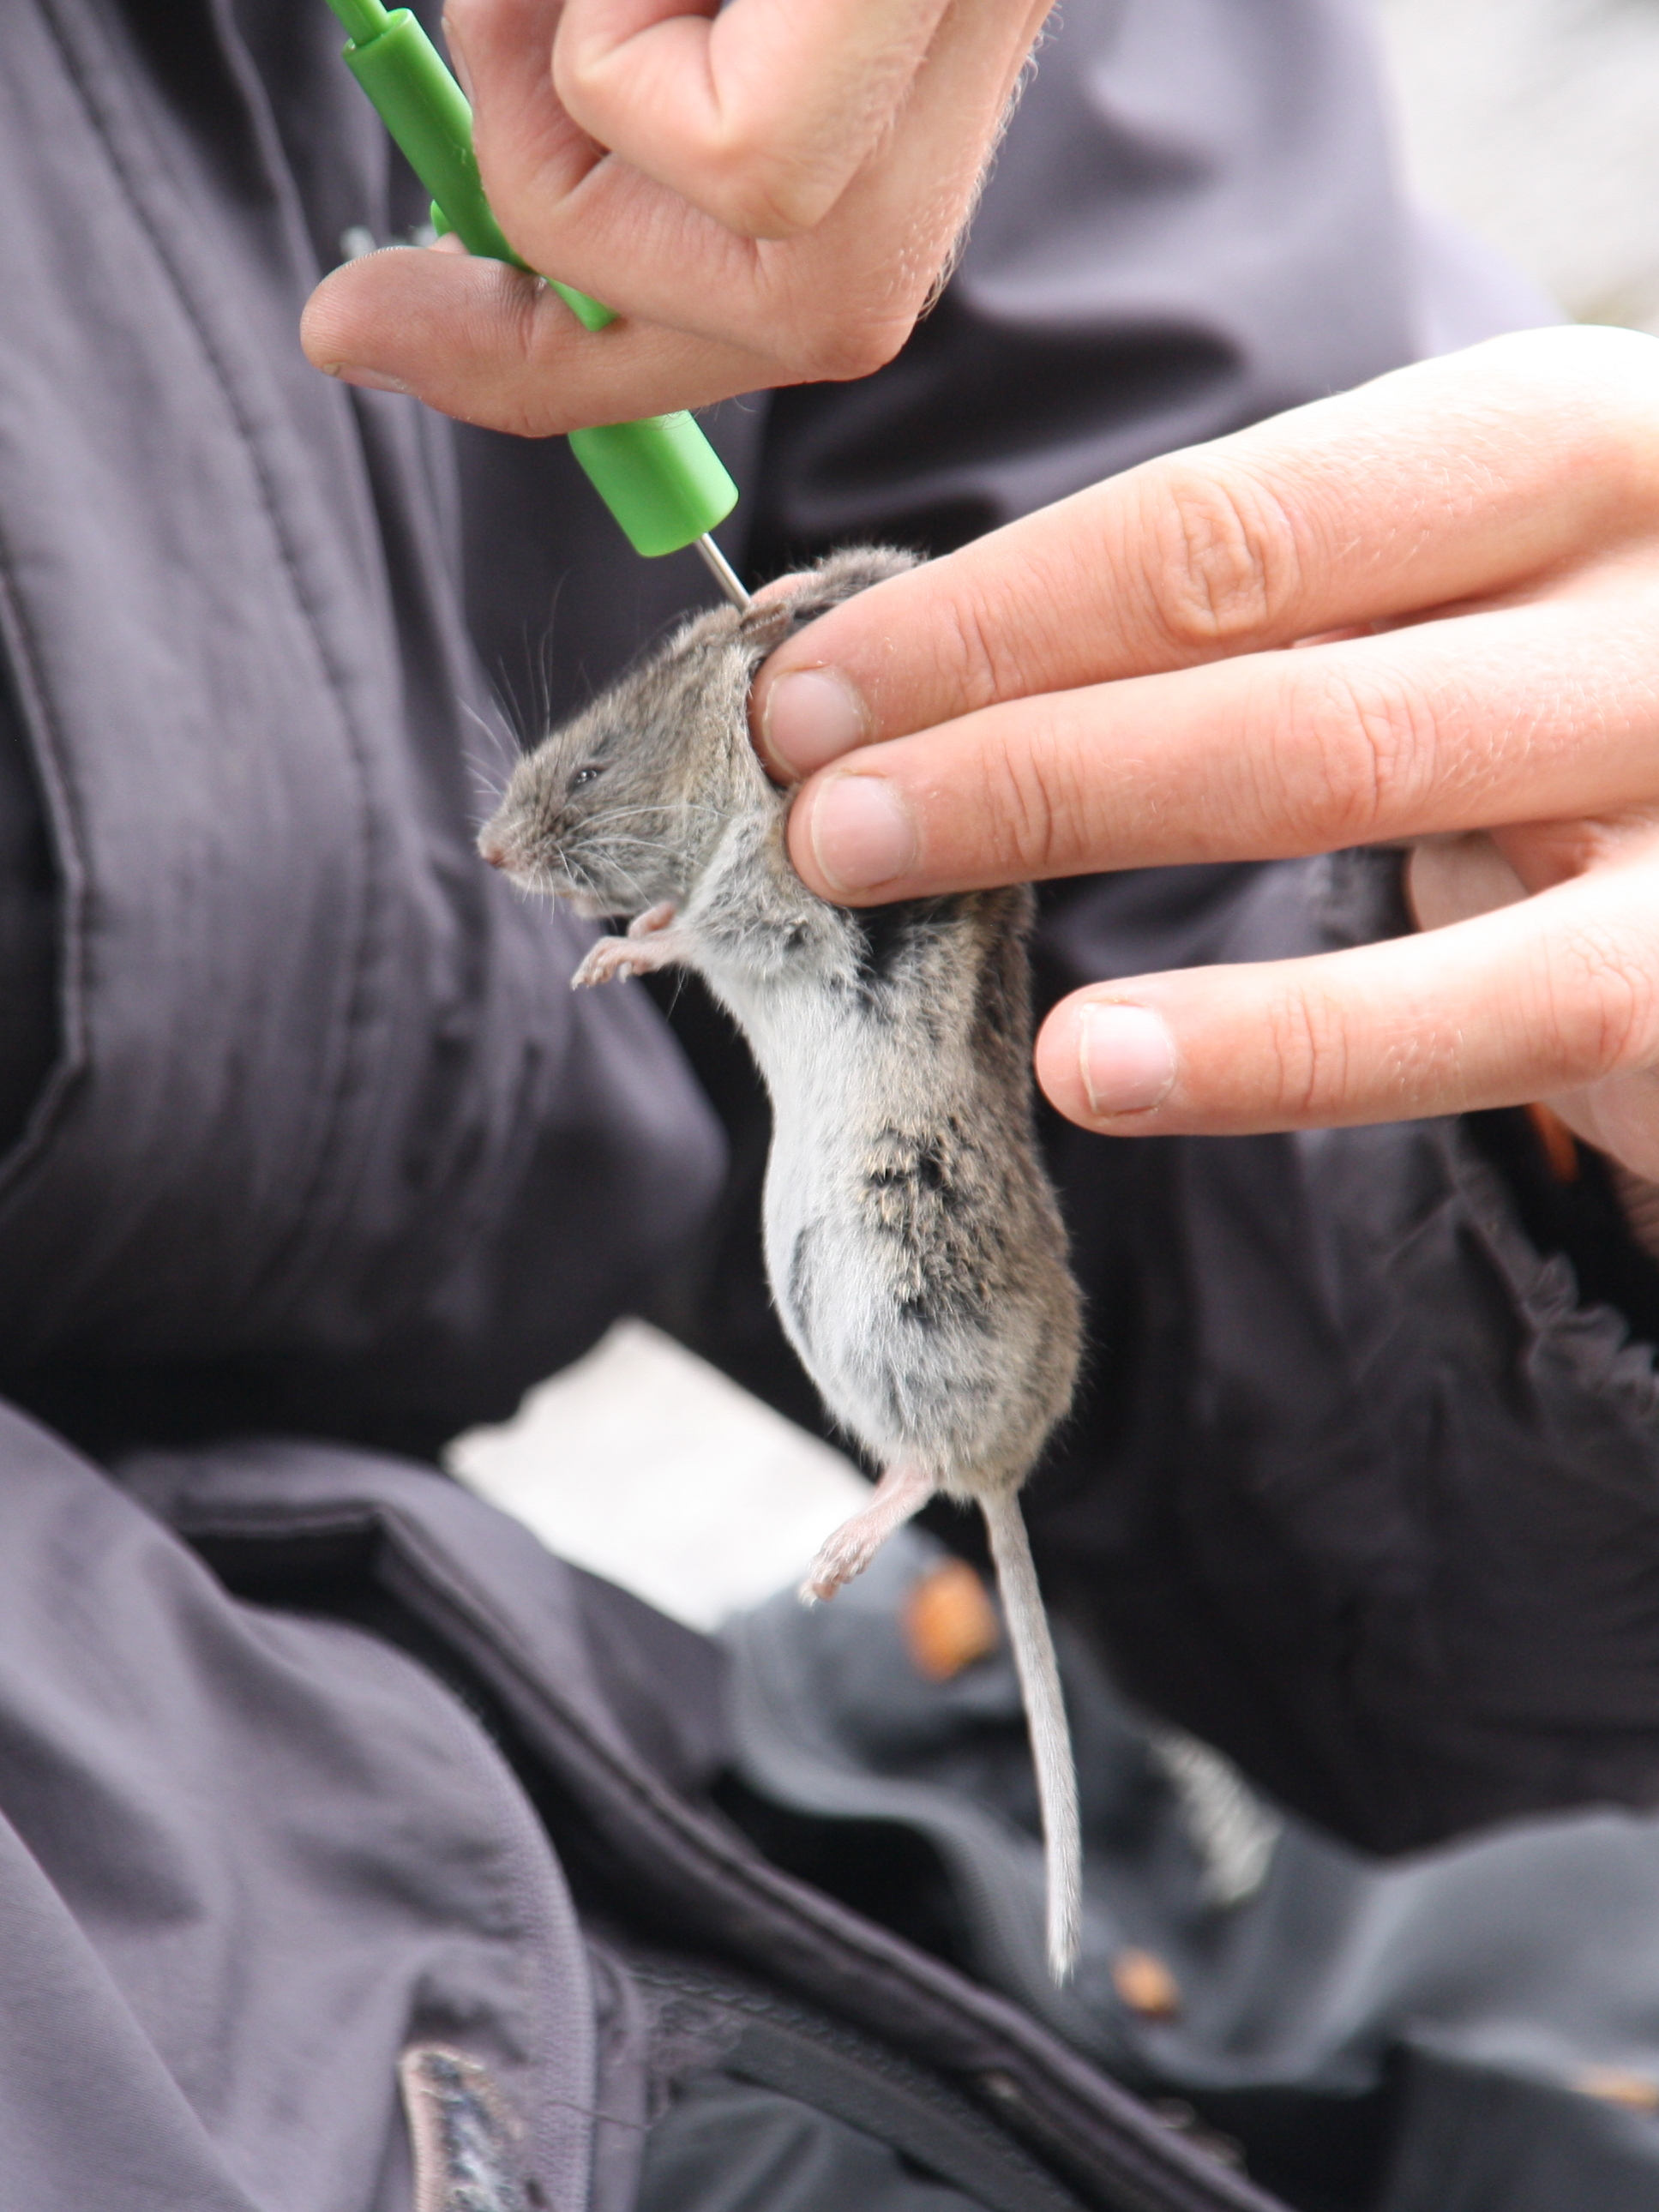
\includegraphics[height= \textheight]{Figures/CN2015_MeulenbroekLiz_00022}}
		\only<4>{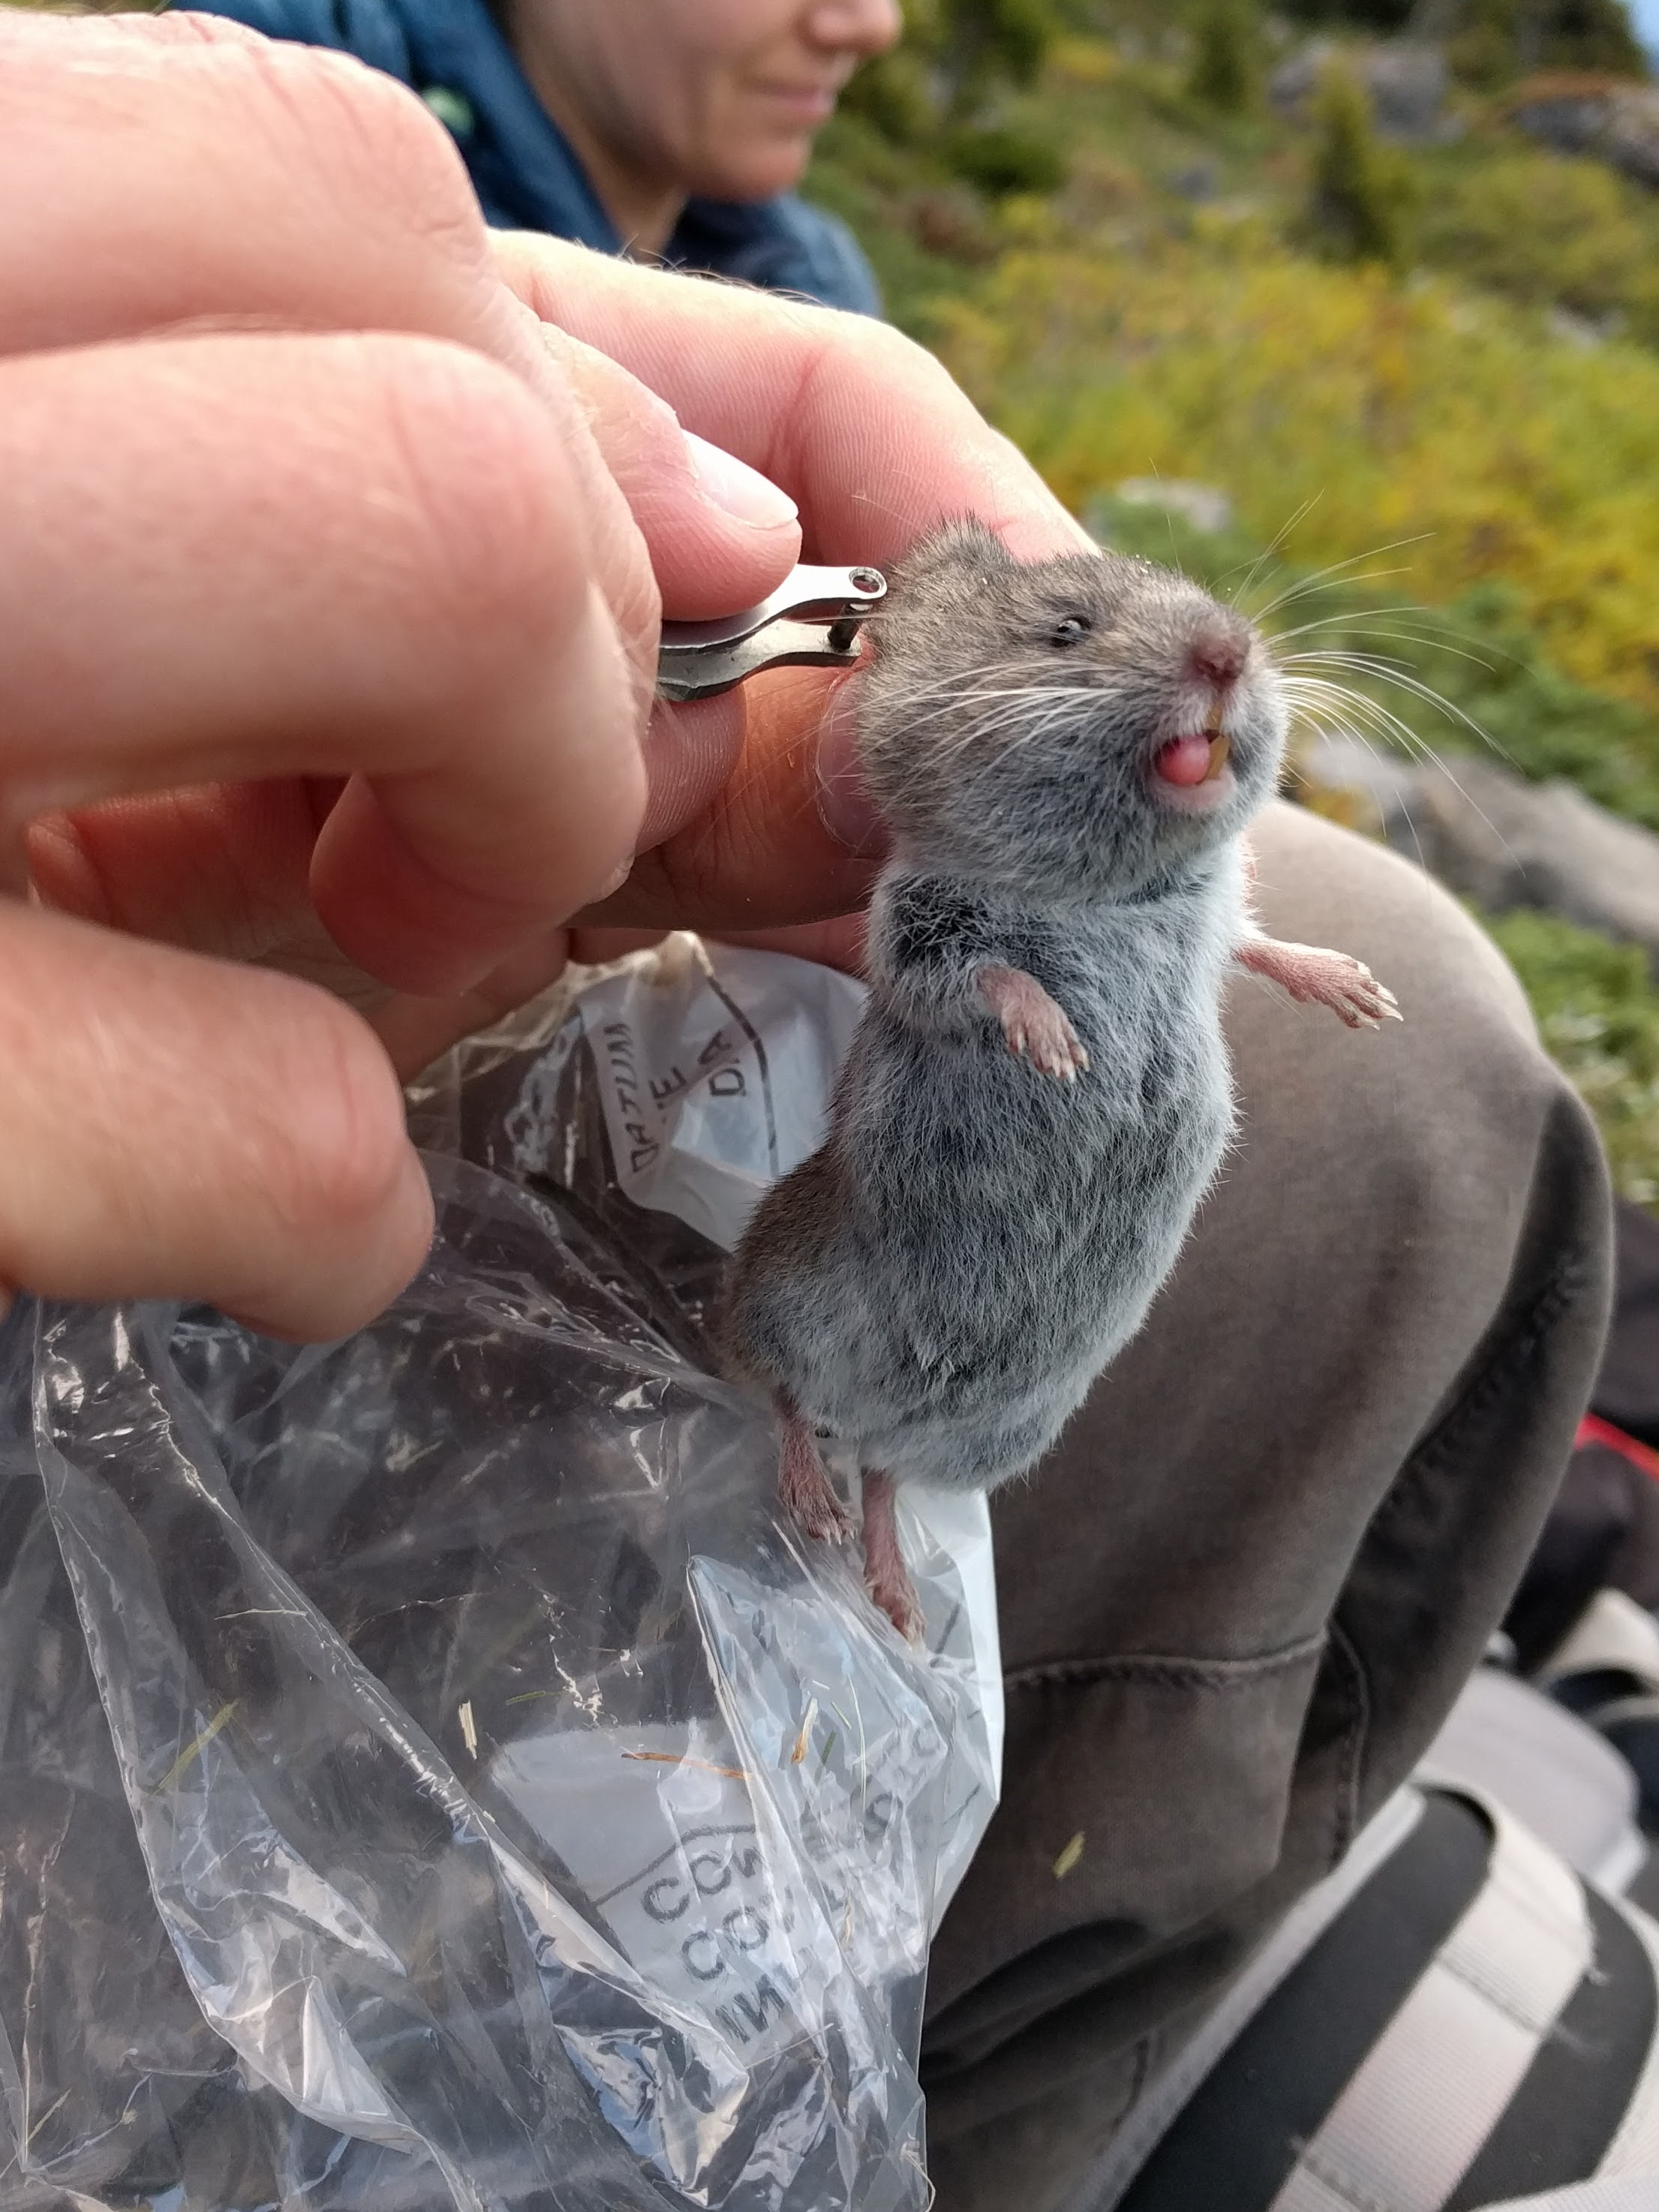
\includegraphics[height= \textheight]{Figures/IMG_20160916_075241}}

	\end{column}
\end{columns}
\end{frame}
%%%%%%%%%%%


%%%%%%%%%%%%%%%%%%%%%%%%%%%%%%%%%%%%%%%%%%%%%%%%%%%%%%
%%%%%%%%%%%%%%%%%%%%%%% Chap 3 %%%%%%%%%%%%%%%%%%%%%%%
%%%%%%%%%%%%%%%%%%%%%%%%%%%%%%%%%%%%%%%%%%%%%%%%%%%%%%

%Open some dice! -> DNA and grass in it, leading to most common number...

%%%%%%%%%%%%%%%%%%%%%%%%%%%%%%%%%%%%%%%%%%%%%%%%%%%%%%
%%%%%%%%%%%%%%%%%%%%%%% Chap 4 %%%%%%%%%%%%%%%%%%%%%%%
%%%%%%%%%%%%%%%%%%%%%%%%%%%%%%%%%%%%%%%%%%%%%%%%%%%%%%



\end{document}
